% !TEX encoding = UTF-8 Unicode
%======================================================================
%  ID5030 — Machine Learning Project Report
%  Group 7 | Gururaj Thorat (ED23B065)
%  Template: ASME asmeconf.cls (mandated by course guidelines)
%======================================================================

\DocumentMetadata{
    lang        = eng-US,
    pdfstandard = A-3u,
    pdfversion  = 1.7,
}

\documentclass[colorlinks,balance]{asmeconf}

% Find figures in the sibling figures/ directory (no need to copy them)
\graphicspath{{../figures/}{./figures/}}

\hypersetup{%
    pdfauthor   = {Gururaj Thorat},
    pdftitle    = {Household Financial Fragility in India: A Composite Index and a Bayesian Early-Warning LSTM},
    pdfkeywords = {financial fragility, IHDS-II, household survey, machine learning, random forest, India},
    pdfsubject  = {ID5030 Course Project Report},
}

\allowdisplaybreaks

%---------------------------------------------------------------------
% Tighten float / caption spacing.
% asmeconf's defaults leave noticeable vertical whitespace above and below
% each figure and table; the values below shrink it without overlap.
%---------------------------------------------------------------------
\setlength{\textfloatsep}{6pt plus 2pt minus 2pt}
\setlength{\floatsep}{6pt plus 2pt minus 2pt}
\setlength{\intextsep}{6pt plus 2pt minus 2pt}
\setlength{\dbltextfloatsep}{6pt plus 2pt minus 2pt}
\setlength{\dblfloatsep}{6pt plus 2pt minus 2pt}
\setlength{\abovecaptionskip}{4pt}
\setlength{\belowcaptionskip}{2pt}
% More lenient float placement so figures fit nearer their references
\renewcommand{\topfraction}{0.9}
\renewcommand{\bottomfraction}{0.9}
\renewcommand{\textfraction}{0.05}
\renewcommand{\floatpagefraction}{0.7}
\renewcommand{\dbltopfraction}{0.9}
\renewcommand{\dblfloatpagefraction}{0.7}

%---------------------------------------------------------------------
% Draft-only "Outline / TODO" boxes.
%   - Set \showoutlinestrue   to keep the planning notes visible.
%   - Set \showoutlinesfalse  to hide every outline box before final
%     submission (the prose around them is untouched).
%---------------------------------------------------------------------
\usepackage[most]{tcolorbox}
\usepackage{comment}
\newif\ifshowoutlines
\showoutlinesfalse   % outline/TODO boxes hidden for the final submission

\ifshowoutlines
  \specialcomment{outline}{%
    \begin{tcolorbox}[enhanced,breakable,
        colback=yellow!8,colframe=orange!70!black,
        boxrule=0.4pt,arc=2pt,
        title=\small Outline\,/\,TODO,fonttitle=\bfseries\small]\small\itshape
  }{\end{tcolorbox}}
\else
  \excludecomment{outline}
\fi

\begin{document}

% Suppress the asmeconf default ASME copyright in the page footer (this is a
% course report, not an ASME submission).
\fancyfoot[RO,RE]{}

%---------------------------------------------------------------------
% Conference headers — kept neutral for a course report
%---------------------------------------------------------------------
\ConfName{ID5030: Machine Learning for Engineering and Science Applications}
\ConfAcronym{ID5030 Project Report}
\ConfDate{May 2026}
\ConfCity{Chennai, India}
\PaperNo{Group 7}

\title{Household Financial Fragility in India: A Composite Index and a Bayesian Early-Warning \NoCaseChange{LSTM}}

\SetAuthors{Gururaj Thorat\affil{1}}
\SetAffiliation{1}{Group~7 \textbullet\ Roll No.\ ED23B065 \textbullet\ Department of Engineering Design, IIT Madras \textbullet\ \texttt{ed23b065@smail.iitm.ac.in}}

\maketitle

\keywords{financial fragility, IHDS-II, household survey, India, logistic regression, random forest, LightGBM, LSTM, Monte-Carlo Dropout, early warning}

%======================================================================
%  ABSTRACT
%======================================================================
\begin{abstract}
Household financial fragility --- the inability to absorb modest income or expense shocks --- is a central determinant of welfare in low- and middle-income economies, yet survey-based measures of it are scarce for Indian households. Using the second wave of the India Human Development Survey (IHDS-II, 2011--12, $N \!=\! 42{,}152$ households), we construct a six-component Financial Fragility Index (FFI) combining debt burden, consumption stress, asset deficit, employment concentration, dependency pressure, and a distress-borrowing flag; components are z-standardised, equally weighted, and quartile-binned into four fragility states. Three classifiers (logistic regression, random forest, isotonic-calibrated LightGBM) predict the binary Fragile/Distressed label from a \emph{disjoint} non-financial covariate set, with a held-out ROC-AUC of 0.751 / 0.754 / \textbf{0.760} respectively and a leave-states-out generalisation AUC of $0.736\!\pm\!0.015$. We then extend the cross-sectional baseline into a \textbf{Bayesian temporal early-warning system} (Sect.~\ref{sec:ew}): a macro-anchored monthly trajectory simulator with Poisson-distributed medical, disaster, and crop-failure shocks builds 24-month per-household panels; a two-layer LSTM with Monte-Carlo Dropout forecasts whether the household will cross the high-fragility threshold in the next three months; and a credible-interval decision rule converts the posterior into a Low / Medium / High triage tier. The LSTM attains a 3-month-ahead ROC-AUC of \textbf{0.982} --- beating naive carry-forward, a per-household Kalman filter, and an NGBoost benchmark --- and the resulting High tier captures 89\% of all stress events at a 97\% per-tier purity.
\end{abstract}

\begin{tcolorbox}[colback=blue!2,colframe=blue!40!black,
    boxrule=0.4pt,arc=1.5pt,left=4pt,right=4pt,top=2pt,bottom=2pt,
    fontupper=\small]
\textbf{Note on AI assistance.} LLMs were used in this project as an aid for code debugging, \LaTeX{} formatting, content refinement and concept clarification.
\end{tcolorbox}

% Fill the rest of the left column with whitespace so the Introduction
% starts at the top of the right column on page 1.
\vfill\null\newpage

%======================================================================
%  1. INTRODUCTION
%======================================================================
\section{Introduction}

\subsection{Background}
\begin{outline}
\textbf{Plan:} one paragraph on what financial fragility means, why it matters in low-/middle-income economies, and how Indian household finance is historically under-instrumented relative to developed economies.\\
\textbf{Status:} drafted below.
\end{outline}
Financial fragility refers to a household's inability to absorb modest, unanticipated income or expense shocks without resorting to high-cost coping mechanisms such as informal borrowing, asset distress sales, or the deferral of essential consumption. In low- and middle-income economies the consequences of such fragility extend well beyond the affected household: weak buffers transmit local shocks into health outcomes, child education, and labour-market participation, and they amplify the impact of macroeconomic disturbances such as inflation, monsoon failure, and global commodity cycles. India is a particularly informative setting for studying household fragility because a large share of consumption is financed out of irregular, informal-sector earnings, formal insurance penetration is low, and credit access is fragmented between commercial banks, cooperatives, microfinance institutions, shopkeeper credit, and unregulated moneylenders. Despite this, household-level survey instrumentation in India has historically focused either on stock-based poverty (income, expenditure quantiles) or on multidimensional deprivation indices, with relatively little attention to flow-based liquidity and shock-absorption.

\subsection{Literature Review}
\begin{outline}
\textbf{Plan:} 2--3 short paragraphs surveying:
\begin{itemize}
\item Lusardi, Schneider, Tufano (2011) -- the original ``financial fragility'' framing using the ``can you raise \$2{,}000 in 30 days?'' benchmark.
\item Studies using IHDS / NSSO / CMIE for household welfare in India.
\item ML-based welfare classification (e.g., Jean et al.\ on poverty from satellite imagery; Blumenstock on mobile-phone metadata).
\item Indices of multidimensional poverty (Alkire--Foster) and how the FFI differs (focuses on flow / shock-absorption, not stock deprivation).
\end{itemize}
\textbf{Status:} drafted below.\\
\textbf{Still to do:} add 1--2 India-specific household-finance citations (e.g.\ Chakrabarty / RBI Household Finance Committee report, NSSO debt and investment survey).
\end{outline}
The modern literature on household financial fragility was crystallised by Lusardi, Schneider, and Tufano~\cite{lusardi2011fragility} via the ``\$2{,}000-in-30-days'' benchmark, which showed nearly half of US households were fragile even before the 2008 crisis. Most cross-country adaptations since remain anchored to single survey questions rather than composite indices over multiple structural risk factors. The multidimensional poverty literature~\cite{alkire2011counting} offers a complementary aggregation methodology --- best known as the Global Multidimensional Poverty Index (MPI) --- but the MPI is built from \emph{stock} indicators of deprivation (schooling, nutrition, sanitation) rather than flow indicators of liquidity and exposure, and is therefore not designed to capture the short-horizon shock-absorption notion at the centre of financial fragility.

A separate strand uses machine learning on non-traditional signals to estimate household welfare: Jean et al.~\cite{jean2016poverty} predicted asset wealth in African villages from satellite imagery, and Blumenstock et al.~\cite{blumenstock2015predicting} predicted poverty from mobile-phone metadata in Rwanda. Both demonstrate that proxies far cheaper than a full household survey can recover much of the welfare signal --- but the analogous question for \emph{financial fragility} in India, whether easily-observed demographic and infrastructural household attributes can identify financially fragile households, has not been systematically addressed.

\subsection{Research Gap and Problem Statement}
Two gaps motivate this work. \textit{First}, there is no widely-adopted composite measure of household financial fragility specific to the Indian context that simultaneously aggregates debt, consumption, assets, employment risk, and recourse to distress borrowing. \textit{Second}, while several studies use ML to predict welfare from alternative data, there is limited evidence on whether non-financial household attributes routinely collected in standard demographic surveys --- housing quality, sanitation, head-of-household education, urban/rural status, caste and religion --- can identify fragile households accurately enough to inform policy targeting where collecting income and debt data at scale is expensive or unreliable. We address both gaps in two stages: stage one constructs a household-level Financial Fragility Index from IHDS-II~\cite{ihds2}, aggregating six standardised components; stage two trains supervised classifiers that predict the binary high-fragility label using a \emph{disjoint} set of non-financial predictors, ensuring no label leakage from the FFI inputs into the predictor matrix.

\subsection{Objectives}
\begin{enumerate}
\item Construct a transparent, reproducible Financial Fragility Index for Indian households using IHDS-II.
\item Classify households into four fragility states (Stable, Stretched, Fragile, Distressed) and a binary high-fragility label.
\item Train and compare a linear (logistic regression) and two non-linear (random forest, gradient-boosted trees) classifiers that predict the binary label from non-financial covariates, with cross-validated hyperparameter selection and probability calibration.
\item Identify the most informative features for distinguishing fragile households, and interpret their policy relevance.
\item Demonstrate, via a macro-anchored synthetic monthly trajectory simulator, how an LSTM with Monte-Carlo Dropout would convert the cross-sectional model into a Bayesian early-warning system that issues Low/Medium/High risk tiers at a three-month forecast horizon (Sect.~\ref{sec:ew}).
\end{enumerate}

%======================================================================
%  2. METHODOLOGY
%======================================================================
\section{Methodology}

\subsection{Data}
\begin{outline}
\textbf{Plan:} describe IHDS-II (round 2, 2011--12), DS0001 individual file, DS0002 household file, sample design (STATEID/DISTID/PSUID/HHID/HHSPLITID keys), national coverage, sample size before and after cleaning. Cite the dataset.\\
Mention \texttt{preprocess\_ihds.py}: merging DS0001 + DS0002 on the five-key household identifier; recoding IHDS missing codes ($-9$, $-8$, $-7$) to NaN.\\
\textbf{Status:} prose drafted below.
\end{outline}
The empirical analysis uses the second wave of the India Human Development Survey (IHDS-II), a nationally representative panel survey of 42{,}152 households across 33 states and union territories, conducted by the National Council of Applied Economic Research and the University of Maryland in 2011--12~\cite{ihds2}. IHDS-II uses a stratified multistage probability sample with the rural and urban frames designed to be self-weighting within strata. We work primarily with the household file (\texttt{DS0002}, $N = 42{,}152$ households) and merge in selected individual-level variables from \texttt{DS0001} ($N = 204{,}569$ individuals) keyed on the five-tuple (\texttt{STATEID}, \texttt{DISTID}, \texttt{PSUID}, \texttt{HHID}, \texttt{HHSPLITID}).

Preprocessing follows two steps implemented in \texttt{preprocess\_ihds.py}. First, the IHDS missing codes $-9$, $-8$, and $-7$ (refused, don't know, and inapplicable, respectively) are converted to \texttt{NaN} so that downstream imputation operates only on genuine missingness. Second, a unique household identifier \texttt{hh\_id} is constructed by concatenating the five merge keys; this identifier links the FFI labels back to the predictor matrix without ambiguity.

\subsection{Financial Fragility Index Construction}
The FFI aggregates six household-level components, each oriented so that higher values indicate \emph{greater} fragility: \textbf{debt burden} $c_1 \!=\! \text{DebtTotal}/(|\text{INCOME}|\!+\!\varepsilon)$, with total debt $=$ \texttt{DB5}$+$\texttt{DB6A}; \textbf{consumption stress} $c_2 \!=\! \text{COTOTAL}/(|\text{INCOME}|\!+\!\varepsilon)$; \textbf{asset deficit} $c_3 \!=\! -\!\log(1\!+\!\max(\text{ASSETS},0))$; \textbf{employment concentration} $c_4 \!=\! \sum_k s_k^2$, the Herfindahl index over five worker-type buckets (non-agricultural, agricultural-labour, salary, business, farm); \textbf{dependency pressure} $c_5 \!=\! \text{NonEarners}/(\text{Earners}\!+\!1)$; and \textbf{distress borrowing} $c_6 \!\in\! \{0,1\}$, flagging households whose largest-loan purpose is consumption or medical, or who borrowed from a shopkeeper or moneylender.

Monetary variables are winsorised at the 1st and 99th percentiles before z-standardisation. The FFI is the equal-weighted mean of the six z-scored components:
\begin{equation}\label{eq:ffi}
\text{FFI}_h = \frac{1}{6}\sum_{j=1}^{6} z\!\left(c_{j,h}\right)
\end{equation}
Households are split into four fragility states using the FFI quartiles: $Q_1$ Stable, $Q_2$ Stretched, $Q_3$ Fragile, $Q_4$ Distressed. The binary supervised label is
\begin{equation}\label{eq:fragbinary}
y_h = \mathbb{1}\{\text{State}_h \in \{\text{Fragile}, \text{Distressed}\}\}.
\end{equation}

\subsection{Predictor Variables}
\begin{outline}
\textbf{Plan:} list the predictor blocks used in \texttt{training\_baseline.py} and emphasize that they are \emph{disjoint from FFI inputs}: head demographics, education, social identity, geography, housing quality, services, migration. Justify the leakage-prevention choice in one sentence.\\
\textbf{Status:} drafted below.
\end{outline}
The predictor matrix is deliberately disjoint from the variables that enter the FFI in Eqs.~\eqref{eq:ffi}--\eqref{eq:fragbinary}: no income, consumption, asset, debt, or worker-type column appears as a predictor. This separation guarantees that the supervised problem cannot trivially recover the label from its own inputs, and that the classifier's accuracy is informative about the predictive content of \emph{non-financial} household attributes. The predictor blocks are: \textbf{head demographics} (\texttt{MHEADAGE}, \texttt{FHEADAGE}); \textbf{head education} (\texttt{HHEDUC}, \texttt{HHEDUCM}, \texttt{HHEDUCF}); \textbf{social identity} (\texttt{ID11} caste, \texttt{ID13} religion, \texttt{GROUPS}); \textbf{geography} (\texttt{URBAN2011}, \texttt{URBAN4\_2011}, \texttt{METRO}, \texttt{METRO6}); \textbf{housing quality} (\texttt{HQ1}, \texttt{HQWALL}, \texttt{HQROOF}, \texttt{HQFLOOR}); \textbf{water/sanitation/kitchen/cooking fuel} (\texttt{WATER}, \texttt{SATOILET}, \texttt{SAKITCHEN}, \texttt{FU1}, \texttt{FULPG}); and \textbf{migration history} (\texttt{MG1}). Categorical IHDS codes are one-hot encoded with an explicit \texttt{NaN} indicator column (\texttt{dummy\_na=True}), so that ``missing'' is treated as its own informative category rather than being silently imputed away.

\subsection{Models and Training Protocol}
We use a stratified 80/20 train/test split (\texttt{random\_state} 42) on $N \!=\! 42{,}152$ households. All hyperparameter selection runs on 5-fold stratified cross-validation over the \emph{training} fold only; the held-out 8{,}431-row test set is touched once, at evaluation, to produce Table~\ref{tab:metrics}. Three classifiers are compared: \textbf{logistic regression} (median imputation $\to$ \texttt{StandardScaler(with\_mean=False)} $\to$ \texttt{LogisticRegression} with $C \!\in\! \{0.1, 1, 5\}$ selected by CV AUC); \textbf{random forest} (median imputation $\to$ 400 trees, \texttt{min\_samples\_leaf}$=$20, no depth limit, \texttt{random\_state}$=$42); and \textbf{gradient-boosted trees (LightGBM)}~\cite{ke2017lightgbm} with native NaN handling, a $\{31, 63, 127\}\!\times\!\{50, 100\}$ \texttt{num\_leaves}/\texttt{min\_child\_samples} grid by CV AUC, learning rate $0.05$, and early stopping (50 rounds) on a held-out 15\% validation slice (final config: \texttt{num\_leaves}$=$31, \texttt{min\_child\_samples}$=$50, 167 trees). The LightGBM model is also isotonic-calibrated via \texttt{CalibratedClassifierCV} with 5-fold CV. We report precision, recall, F1, ROC-AUC, average precision (AP), and the Brier score on the held-out test split at the default classification threshold of 0.5; calibration is evaluated by the Brier score and by reliability diagrams (Fig.~\ref{fig:calib}). To probe sensitivity, three robustness checks (Sect.~\ref{sec:robustness}) replace (i)~equal weights with a PCA-derived weighting, (ii)~the median cutoff with a top-tertile cutoff, and (iii)~the random test fold with a leave-states-out GroupKFold by \texttt{STATEID}. Feature attribution uses tree-explained SHAP values~\cite{lundberg2017shap} on a 3{,}000-row test sample; impurity-based importance is biased toward high-cardinality variables~\cite{strobl2007bias} and reported only for transparency.

%======================================================================
%  3. RESULTS AND DISCUSSION
%======================================================================
\section{Results and Discussion}

\subsection{Fragility Distribution}
After winsorisation and equal-weighted z-score aggregation of the six components, the FFI has mean 0 and standard deviation 0.41 by construction; its empirical distribution is strongly right-skewed (sample skewness $\approx 17.5$), with a small tail of households whose debt and consumption ratios are extreme multiples of income (Fig.~\ref{fig:ffi_dist}). The quartile binning therefore produces four well-defined groups: Stable ($n\!=\!10{,}529$), Stretched ($n\!=\!10{,}528$), Fragile ($n\!=\!10{,}528$), and Distressed ($n\!=\!10{,}567$), and the binary high-fragility label is consequently balanced at 50.0/50.0.

The composition of these groups is markedly different across urban and rural India. Rural households account for 54.7\% of the Fragile/Distressed pool, against only 41.2\% in the urban subsample (Fig.~\ref{fig:urban_rural}); equivalently, a rural household is roughly one-third more likely to land in the high-fragility half of the distribution than an urban household. The state-level breakdown (Fig.~\ref{fig:by_state}) shows a similarly large spread: states in the eastern and central belt --- Bihar, Jharkhand, Madhya Pradesh, Chhattisgarh, Odisha --- carry the highest Fragile/Distressed shares (well above 60\%), while the southern and far-northern states (Kerala, Goa, Himachal Pradesh, Jammu \& Kashmir) sit at the other end. These spatial patterns are consistent with the headline poverty geography of India and reassure that the FFI is not capturing pure noise.

\begin{figure}[!htb]
\centering
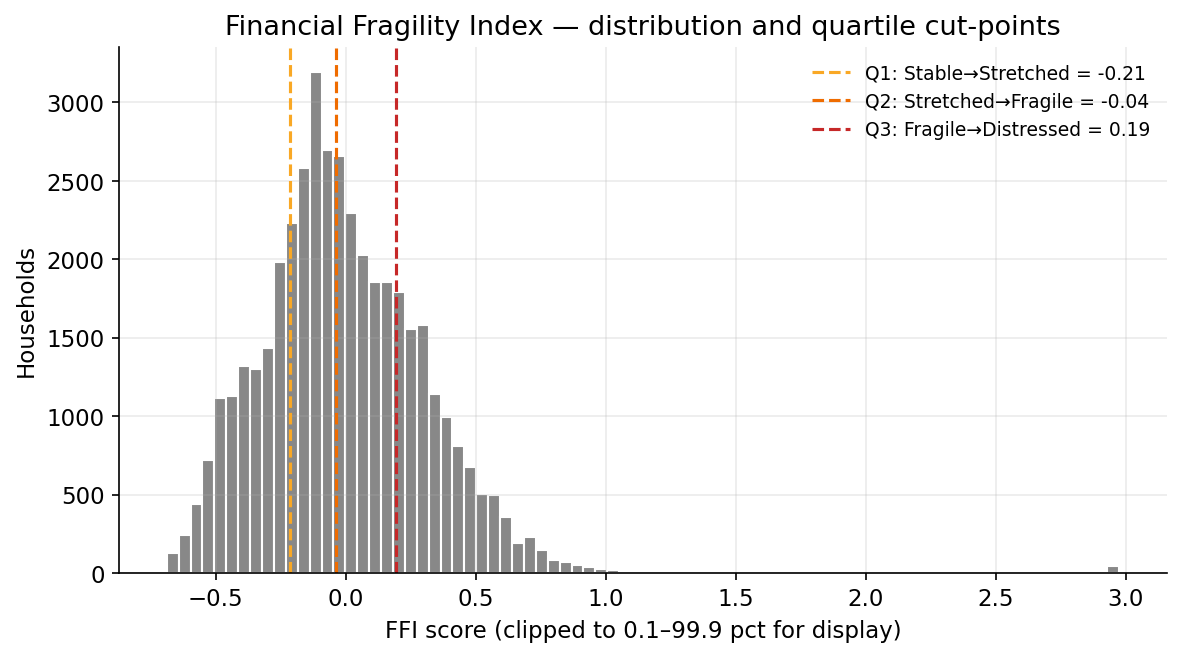
\includegraphics[width=0.95\linewidth]{01_ffi_distribution.png}
\caption{Distribution of the Financial Fragility Index across IHDS-II households. The right tail is heavy because the debt-to-income and consumption-to-income components are themselves heavy-tailed even after 1\%/99\% winsorization.}\label{fig:ffi_dist}
\end{figure}

\begin{figure}[!htb]
\centering
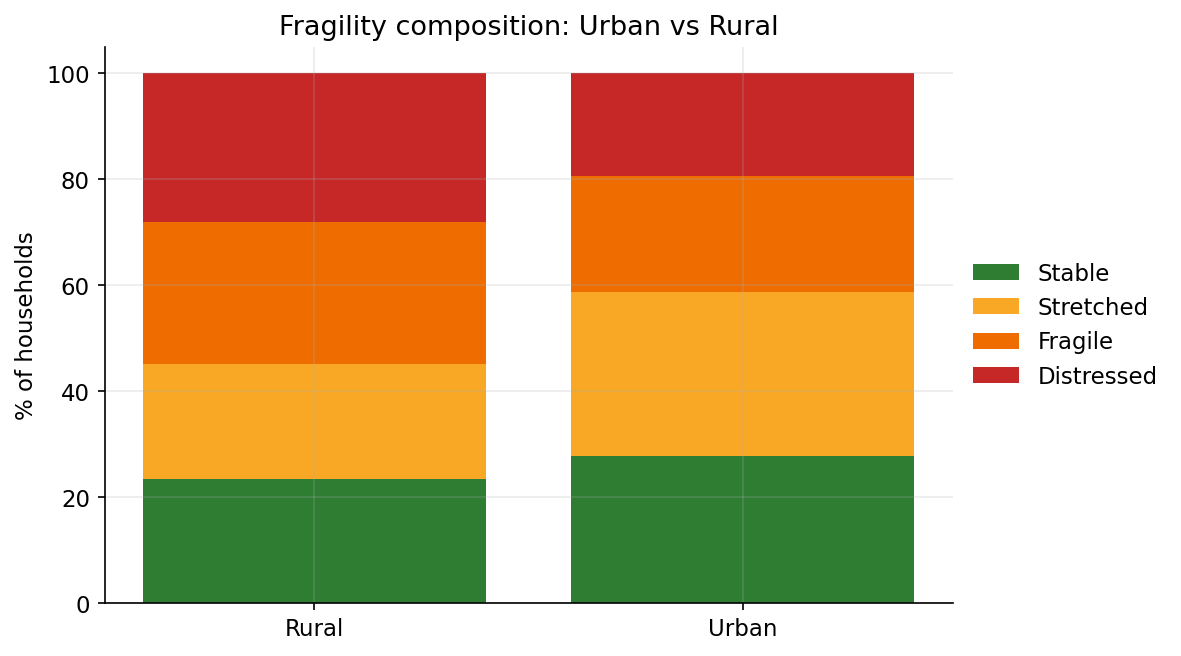
\includegraphics[width=0.95\linewidth]{04_fragility_by_urban_rural.png}
\caption{Share of households in each fragility state, by urban/rural location. 54.7\% of rural households fall in the Fragile or Distressed groups, against 41.2\% of urban households.}\label{fig:urban_rural}
\end{figure}

\begin{figure}[!htb]
\centering
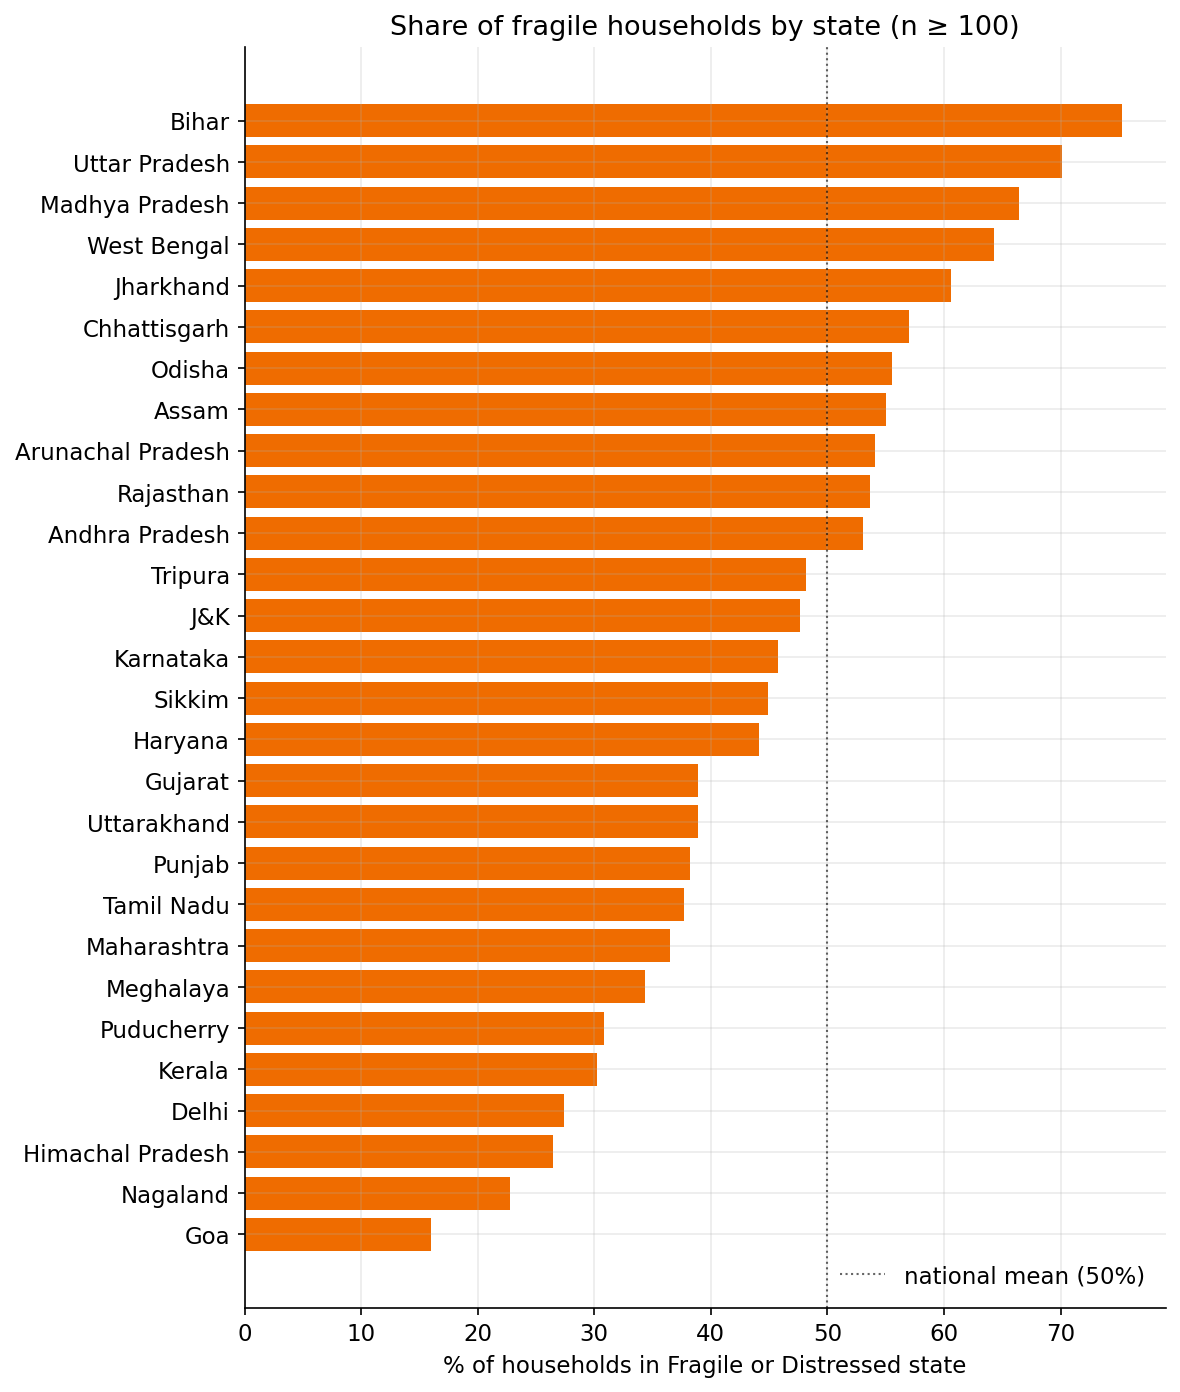
\includegraphics[width=0.95\linewidth]{05_fragility_by_state.png}
\caption{State-wise share of Fragile/Distressed households. The eastern and central belt is consistently above the national share; the southern and far-northern states sit below it.}\label{fig:by_state}
\end{figure}

\subsection{Classifier Performance}
Held-out test-set performance is summarised in Table~\ref{tab:metrics}. All three classifiers achieve a ROC-AUC in the 0.75--0.76 range on the disjoint non-financial covariate set, comfortably above the 0.5 chance baseline implied by the balanced binary label. The relative ordering --- LightGBM $>$ Random Forest $>$ Logistic Regression --- is consistent across CV, the held-out test set, and the average-precision metric (Fig.~\ref{fig:pr}), and the gap between LightGBM (AUC 0.760 after isotonic calibration) and logistic regression (0.751) is small but reproducible across the five CV folds. Isotonic calibration of LightGBM reduces the Brier score from 0.200 to 0.199 and visibly tightens the reliability diagram in the upper half of the predicted-probability range (Fig.~\ref{fig:calib}); the raw LightGBM model was already approximately well-calibrated, so the gains are modest.

At the default 0.5 threshold the calibrated LightGBM correctly identifies 67.3\% of Fragile/Distressed households with 70.5\% precision (Fig.~\ref{fig:cm}). The confusion matrices are nearly symmetric across all three models, indicating that the residual error is not driven by class imbalance but by genuine overlap of the covariate distributions of Fragile and non-Fragile households in the lower-middle range of the FFI.

\begin{table*}[!htb]
\caption{Held-out test-set classification performance for the binary Fragile/Distressed label, $N_{\text{test}}\!=\!8{,}431$. Operating threshold $\!=\!0.5$. 5-fold CV AUC is computed on the training fold ($N_{\text{train}}\!=\!33{,}721$). AP $=$ average precision.}\label{tab:metrics}
\centering
\tagpdfsetup{table/header-rows={1}}%
\begin{tabular}{lcccccc}
\toprule
Model & Precision & Recall & F1 & ROC-AUC & AP & Brier \\
\midrule
Logistic Regression       & 0.695 & 0.670 & 0.683 & 0.751 & 0.748 & 0.203 \\
Random Forest             & 0.701 & 0.673 & 0.686 & 0.754 & 0.752 & 0.202 \\
LightGBM                  & 0.703 & 0.672 & 0.687 & 0.759 & 0.758 & 0.200 \\
LightGBM (isotonic)       & \textbf{0.705} & \textbf{0.673} & \textbf{0.689} & \textbf{0.760} & \textbf{0.758} & \textbf{0.199} \\
\midrule
\multicolumn{4}{l}{LightGBM, 5-fold CV (train)} & \multicolumn{2}{c}{$0.749 \pm 0.007$ (AUC, AP)} & --- \\
\bottomrule
\end{tabular}
\end{table*}

\begin{figure}[!htb]
\centering
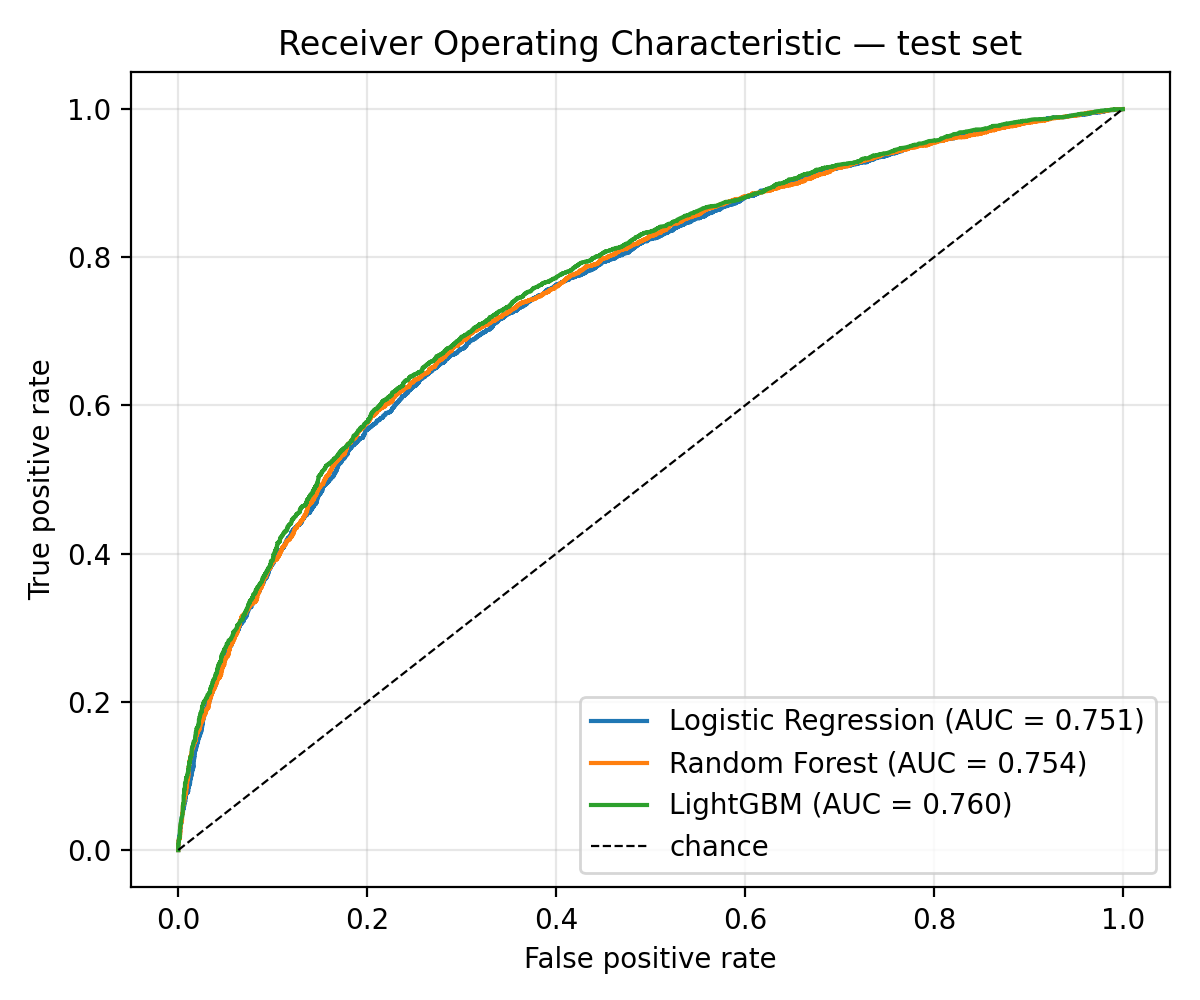
\includegraphics[width=0.95\linewidth]{06_roc_curves.png}
\caption{ROC curves on the held-out test set. The three classifiers track each other closely; LightGBM (after isotonic calibration) is slightly above the random forest, which is in turn slightly above logistic regression.}\label{fig:roc}
\end{figure}

\begin{figure}[!htb]
\centering
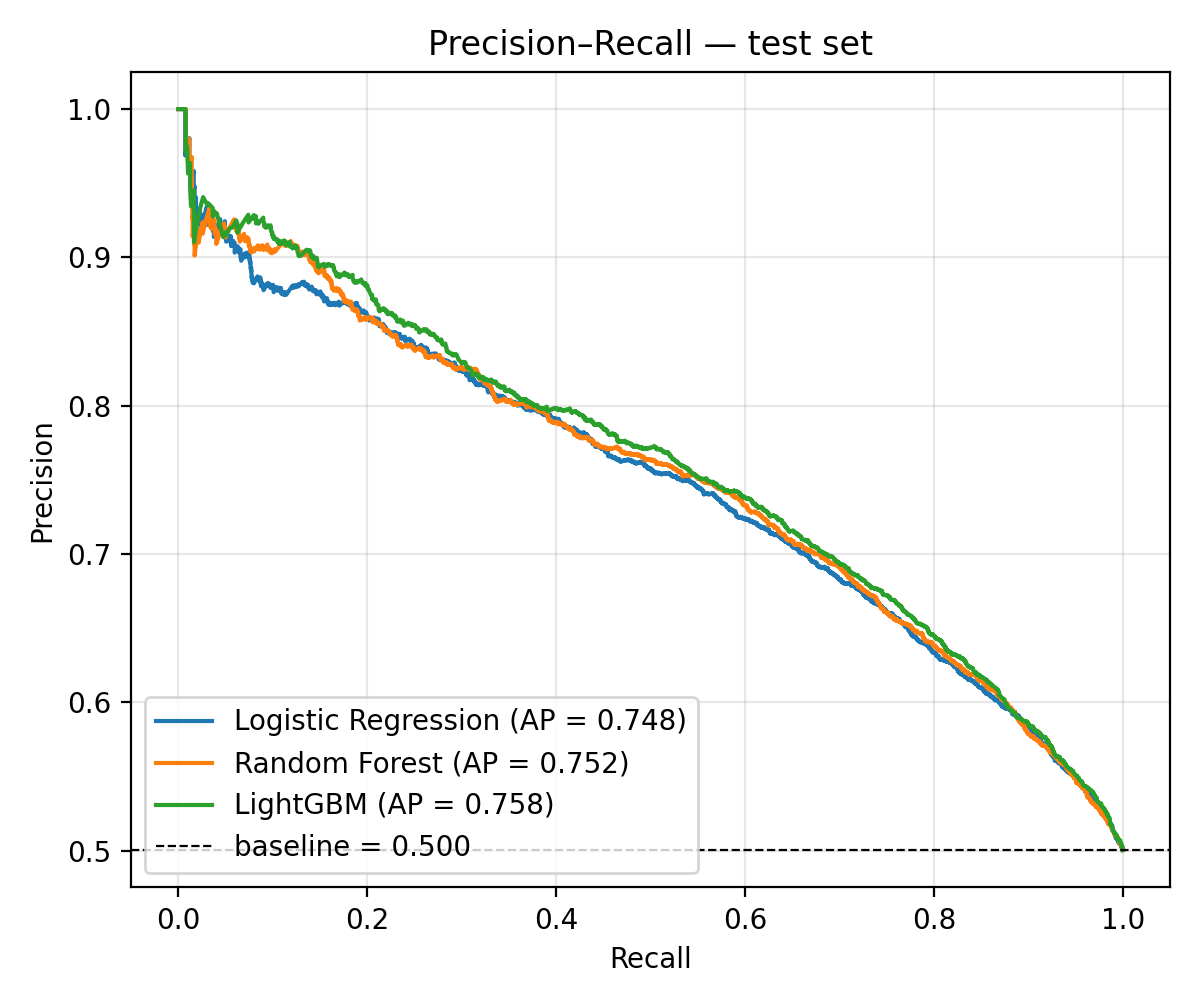
\includegraphics[width=0.95\linewidth]{07_pr_curves.png}
\caption{Precision--recall curves on the held-out test set. The dashed line marks the prevalence baseline (\,$\pi\!=\!0.500$).}\label{fig:pr}
\end{figure}

\begin{figure}[!htb]
\centering
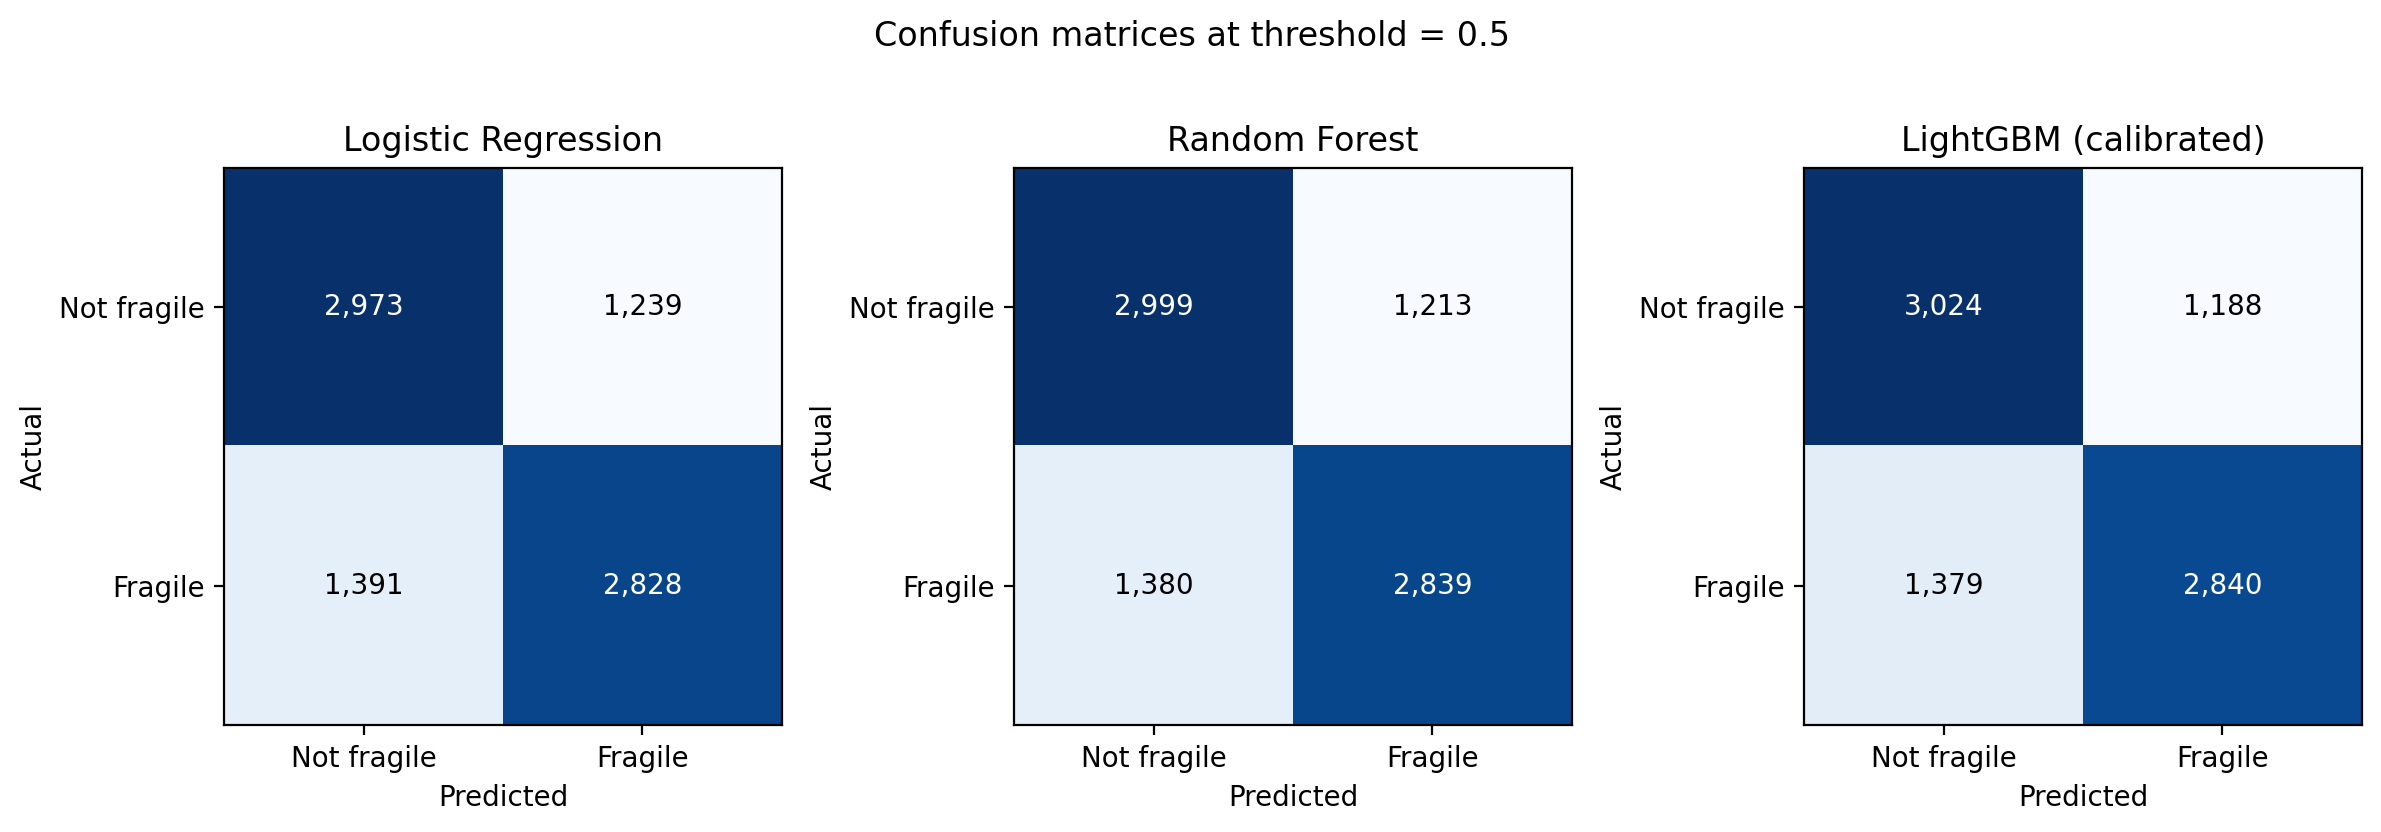
\includegraphics[width=0.95\linewidth]{08_confusion_matrices.png}
\caption{Confusion matrices at threshold 0.5 for the three classifiers.}\label{fig:cm}
\end{figure}

\begin{figure}[!htb]
\centering
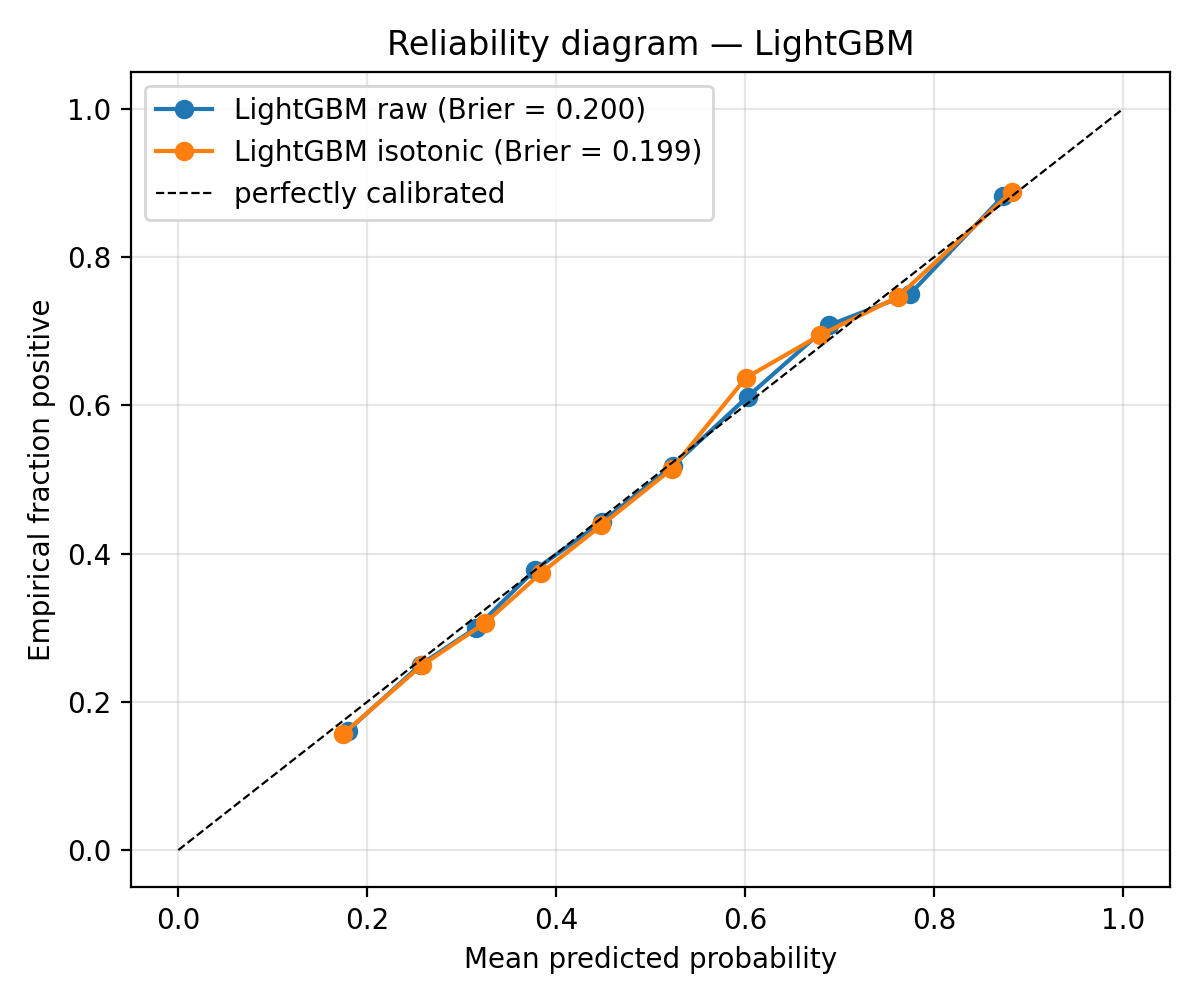
\includegraphics[width=0.95\linewidth]{11_calibration.png}
\caption{Reliability diagram for LightGBM, raw vs.\ isotonic-calibrated, with empirical fraction positive over quantile-spaced predicted-probability bins. Isotonic calibration mildly improves the Brier score (0.200 $\to$ 0.199).}\label{fig:calib}
\end{figure}

\subsection{Feature Importance}\label{sec:shap}
SHAP attribution on the LightGBM model (Fig.~\ref{fig:shap}) and permutation importance on the random forest agree closely. Three thematic blocks dominate. \textbf{Kitchen and cooking-fuel infrastructure} (\texttt{FULPG}, \texttt{FU1}, \texttt{SAKITCHEN}) accounts for the largest share of attribution, with LPG access the single most informative variable. \textbf{Housing-quality indicators} (\texttt{HQFLOOR}, \texttt{HQWALL}, \texttt{HQROOF}) form a tightly correlated, highly informative block. \textbf{Head's demographic and human-capital signals} (\texttt{FHEADAGE}, \texttt{HHEDUCM}, \texttt{HHEDUC}) add an orthogonal source of signal not picked up by the housing block. Sanitation, urban/rural, and social-identity dummies sit further down but remain consistently positive. We adopt SHAP as the headline interpretation because its magnitudes are local additive contributions and are not biased by feature cardinality, unlike impurity-based importance~\cite{strobl2007bias}.

\begin{figure}[!htb]
\centering
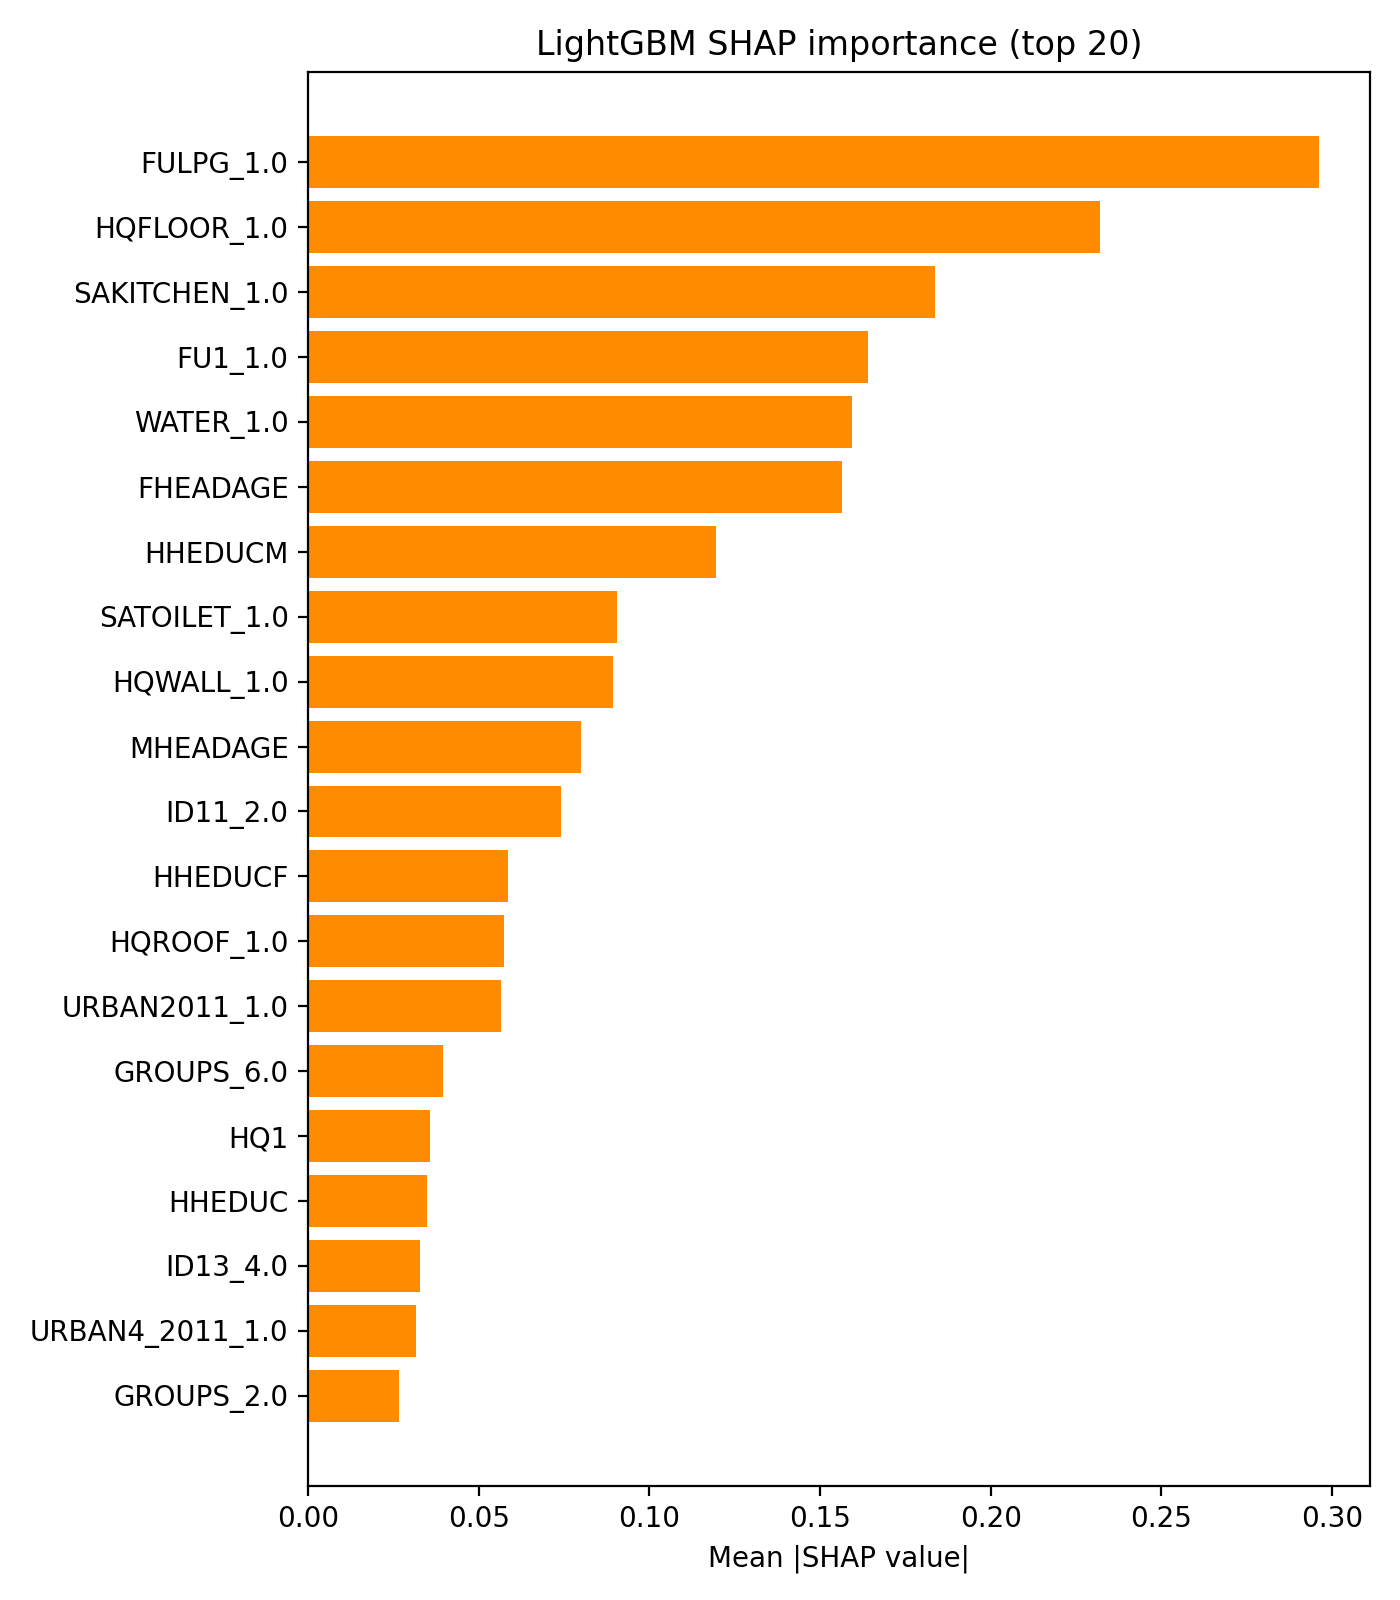
\includegraphics[width=0.92\linewidth]{12_shap_top20.png}
\caption{Top-20 features by mean absolute SHAP value (LightGBM, evaluated on 3{,}000 random test-set rows). LPG use, floor and kitchen quality dominate, followed by water source, head-of-household age, and head's education.}\label{fig:shap}
\end{figure}

\subsection{Robustness}\label{sec:robustness}
Three checks probe the FFI and the LightGBM classifier. \textbf{(a)~PCA versus equal weights.} The first principal component of the six z-scored components correlates with the equal-weight FFI at Pearson $+0.54$ but Spearman $-0.41$; binarising each at its own median yields only 33.6\% agreement (Cohen's $\kappa\!=\!-0.33$). The reason is mechanical: PCA loads disproportionately onto the two heavy-tailed monetary ratios (debt-burden 0.62, consumption-stress 0.66; sample skewness 40.7 vs.\ 17.5 for equal weights), in effect ranking households by debt-to-income alone, while equal weights give each of the six structural dimensions a $\tfrac{1}{6}$ share regardless of natural variance. We therefore retain equal weights as the headline aggregator. \textbf{(b)~Alternative cutoff.} Tightening from a top-half cutoff (prevalence 0.50) to a top-tertile cutoff (prevalence 0.33) reduces the LightGBM test AUC marginally from 0.758 to 0.751; AP drops from 0.757 to 0.618 (mechanical, since AP scales with the positive prevalence). The AUC stability confirms the classifier's discriminative ordering is not an artefact of the median cut. \textbf{(c)~Geographic out-of-sample.} A 5-fold GroupKFold by \texttt{STATEID} --- no state in both training and validation --- yields a mean LightGBM AUC of $0.736 \pm 0.015$, only $\approx\!0.024$ below the in-distribution AUC, indicating the model is not memorising state-specific fixed effects.

\subsection{Discussion}
The classifiers achieve a held-out AUC of $\approx\!0.75$--$0.76$ on a covariate set that contains no income, debt, consumption, asset, or worker-type variable: a checklist of housing-quality, sanitation, cooking-fuel, and head demographic items --- routinely collected in the Census, NSSO, and NFHS --- recovers most of the predictive content that a full financial questionnaire would yield, a useful margin for targeted programme delivery where collecting income or debt at scale is expensive. Two patterns in the residual error are worth flagging: \textit{(i)}~the confusion matrices in Fig.~\ref{fig:cm} are nearly symmetric, so the model neither over- nor under-predicts fragility on average; and \textit{(ii)}~the SHAP analysis shows that the dominant predictors are not the social-identity (caste/religion) variables but the infrastructural ones --- a non-obvious finding suggesting that residual identity-related signal is largely mediated through the housing-and-services bundle. Section-level limitations (single survey wave, FFI aggregation choices, calibration of the operating threshold) are consolidated in Sect.~\ref{sec:conclusion}.

%======================================================================
%  4. TEMPORAL EARLY-WARNING EXTENSION
%======================================================================
\section{Temporal Early-Warning Extension}\label{sec:ew}

\subsection{Motivation}\label{sec:ew:motiv}
The cross-sectional classifier (Sect.~\ref{sec:shap}) identifies households that are \emph{currently} fragile, but early intervention requires predicting the \emph{transition} into stress months ahead from a household's recent financial history --- not observable directly in single-wave IHDS-II. We therefore (i)~build a household-level monthly trajectory by anchoring the IHDS-II annual snapshot to a real macroeconomic series and injecting empirically-calibrated stochastic shocks (Sect.~\ref{sec:ew:sim}); (ii)~define a time-varying $\mathrm{FFI}_t$ via the project plan's flow-based formula (Sect.~\ref{sec:ew:ffit}); and (iii)~train an LSTM with Monte-Carlo Dropout to produce a 3-month-ahead posterior over both $\mathrm{FFI}_{t+3}$ and the binary stress event (Sects.~\ref{sec:ew:lstm}--\ref{sec:ew:mcd}). The headline model is benchmarked against three baselines (Sect.~\ref{sec:ew:bsl}) and converted into a Bayesian Low / Medium / High risk-tier rule (Sect.~\ref{sec:ew:tier}). The synthetic panel is an extrapolation of the cross-sectional anchor under structural assumptions; conclusions of this section should be read as a methodology demonstration of how the early-warning system would be deployed on a real Indian monthly panel (e.g. CMIE CPHS), not as a calibrated forecast for any individual household.

\subsection{Macro-Anchored Trajectory Simulator}\label{sec:ew:sim}
Let $h$ index households and $t \in \{1, \ldots, T\}$, $T = 24$, index months from January~2011 to December~2012 --- the IHDS-II survey window. We denote the household's IHDS-II annual anchors $Y_h$ (\texttt{INCOME}), $C_h$ (\texttt{COTOTAL}), $A_h$ (\texttt{ASSETS}), and initial debt $D_h^{(0)} = \texttt{DB5}_h + \texttt{DB6A}_h$. The real India CPI-Combined series $\{\mathrm{CPI}_t\}_{t=1}^{T}$ (Fig.~\ref{fig:cpi}) is rebased to an anchor month $t^\star$ corresponding to mid-survey (January 2012), so the multiplicative price factor is $m_t \!=\! \mathrm{CPI}_t / \mathrm{CPI}_{t^\star}$.

\paragraph{Income.} The household's monthly income $y_h(t)$ follows a multiplicative log-normal walk around its annualised anchor, modulated by CPI and damped by a binary crop-failure shock indicator $S^{\text{crop}}_h(t)$:
\begin{equation}\label{eq:y}
    y_h(t) = \frac{Y_h}{12}\, m_t \, \exp\!\Big(\epsilon^y_h(t) - \tfrac{1}{2}\sigma^{y}_{h}{}^{2}\Big)\,\big(1 - \delta^{\text{crop}}_h(t) \cdot S^{\text{crop}}_h(t)\big),
\end{equation}
with $\epsilon^y_h(t) \!\sim\! \mathcal{N}(0, \sigma^y_h{}^2)$ i.i.d.\ across $t$, and the crop-failure income drop $\delta^{\text{crop}}_h(t) \!\sim\! \mathcal{U}(0.30, 0.70)$. The household-specific volatility $\sigma^y_h$ is parameterised from the IHDS-II earner mix: sole-earner farm or agricultural-labour households carry the highest $\sigma^y_h$ (high-variance livelihoods), while salary-majority households carry the lowest. Concretely,
\begin{equation}\label{eq:sigmay}
\begin{aligned}
\sigma^y_h \;=\; \mathrm{clip}\big(\, b_h\, (1 \!+\! \tfrac{1}{2}(\mathcal{H}_h \!-\! \tfrac{1}{5})),\; 0.05,\; 0.45 \big),
\end{aligned}
\end{equation}
with base volatility
\begin{equation}\label{eq:basevol}
\begin{aligned}
b_h \;=\;& 0.10\,\mathbb{I}\{\text{salary maj.}\} \\
        &+\, 0.20\,(1\!-\!\mathbb{I}\{\text{salary maj.}\}) \\
        &+\, 0.10\,\mathbb{I}\{\text{sole farm/aglab}\},
\end{aligned}
\end{equation}
and $\mathcal{H}_h \!=\! \sum_k s_{h,k}^2$ the Herfindahl index over the five worker-type shares.

\paragraph{Expense.} Consumption is smoother than income (consumption smoothing) and carries a deterministic festive bump in October--November and a small lean stretch in March--April. Monthly expense is
\begin{equation}\label{eq:x}
\begin{aligned}
x_h(t) \;=\;& \frac{C_h}{12}\, m_t \, \zeta(t)\, \exp\!\Big(\epsilon^x_h(t) - \tfrac{1}{2}\sigma^{x}{}^2\Big) \\
            &+\; \mathcal{M}^{\text{med}}_h(t)\, S^{\text{med}}_h(t)\;+\; \mathcal{M}^{\text{dis}}_h(t)\, S^{\text{dis}}_h(t),
\end{aligned}
\end{equation}
with $\sigma^x \!=\! 0.10$ (homogeneous), $\epsilon^x_h(t) \!\sim\! \mathcal{N}(0, \sigma^{x}{}^2)$, seasonal $\zeta(t) \!\in\! \{0.95, 1.00, 1.15\}$, and medical / disaster shock magnitudes drawn lognormally from $\log\mathcal{N}(\log(0.5\, Y_h/12),\, 0.8^2)$ and $\log\mathcal{N}(\log(0.3\, Y_h/12),\, 0.6^2)$ respectively.

\paragraph{Shock arrival.} The three shock indicators are independent Bernoulli draws at monthly Poisson rates calibrated from IHDS-II's five-year recall variables in the MI module: $\lambda^{\text{med}} \!=\! \Pr(\texttt{MI1}=1)/60$, $\lambda^{\text{dis}} \!=\! \Pr(\texttt{MI2}=1)/60$, and $\lambda^{\text{crop}} \!=\! \Pr(\texttt{MI5}=1)/60 \!\cdot\! \mathbb{I}\{\text{farm earners} > 0\}$. The calibrated values are $(\lambda^{\text{med}}, \lambda^{\text{dis}}, \lambda^{\text{crop}}) = (0.00441, 0.00131, 0.00264)$, i.e.\ a typical farm household faces $\approx 9.8\%$ probability of at least one shock in any given month (Fig.~\ref{fig:simshock}).

\paragraph{Debt and savings dynamics.} The cash-flow gap in month $t$ is
\begin{equation}\label{eq:gap}
g_h(t) = y_h(t) - x_h(t) - i\, D_h(t\!-\!1),
\end{equation}
where $i = 0.02$ is the monthly debt-service rate (calibrated to $\approx 25\%$ APR on informal credit). Savings $S_h(t)$ absorb negative gaps until exhausted; the residual is rolled into debt. Positive gaps top up savings and repay debt at a fixed split:
\begin{align}
    S_h(t) &= \max\!\big\{0,\; S_h(t\!-\!1) - (g_h(t))^{-} + (g_h(t))^{+} - r_h(t)\big\}, \label{eq:S} \\
    D_h(t) &= \max\!\big\{0,\; D_h(t\!-\!1) + \big[(g_h(t))^{-} - S_h(t\!-\!1)\big]^{+} - r_h(t)\big\}, \label{eq:D}
\end{align}
with $r_h(t) = \min\{0.3\,(g_h(t))^{+},\, D_h(t\!-\!1)\}$ and $(x)^{+} \!=\! \max(x,0)$, $(x)^{-} \!=\! \max(-x,0)$. The initial savings buffer is $S_h(0) = 0.05\, A_h$.

The simulator (\texttt{early\_warning/simulator.py}) produces a long-format panel of $42{,}152 \!\times\! 24 \!=\! 1{,}011{,}648$ rows. By construction the simulated 24-month sums recover the IHDS-II annual anchors to within Monte-Carlo error; realised shock incidence matches the calibrated Poisson targets across all three shock types (Fig.~\ref{fig:simshock}).

\begin{figure}[!htb]
\centering
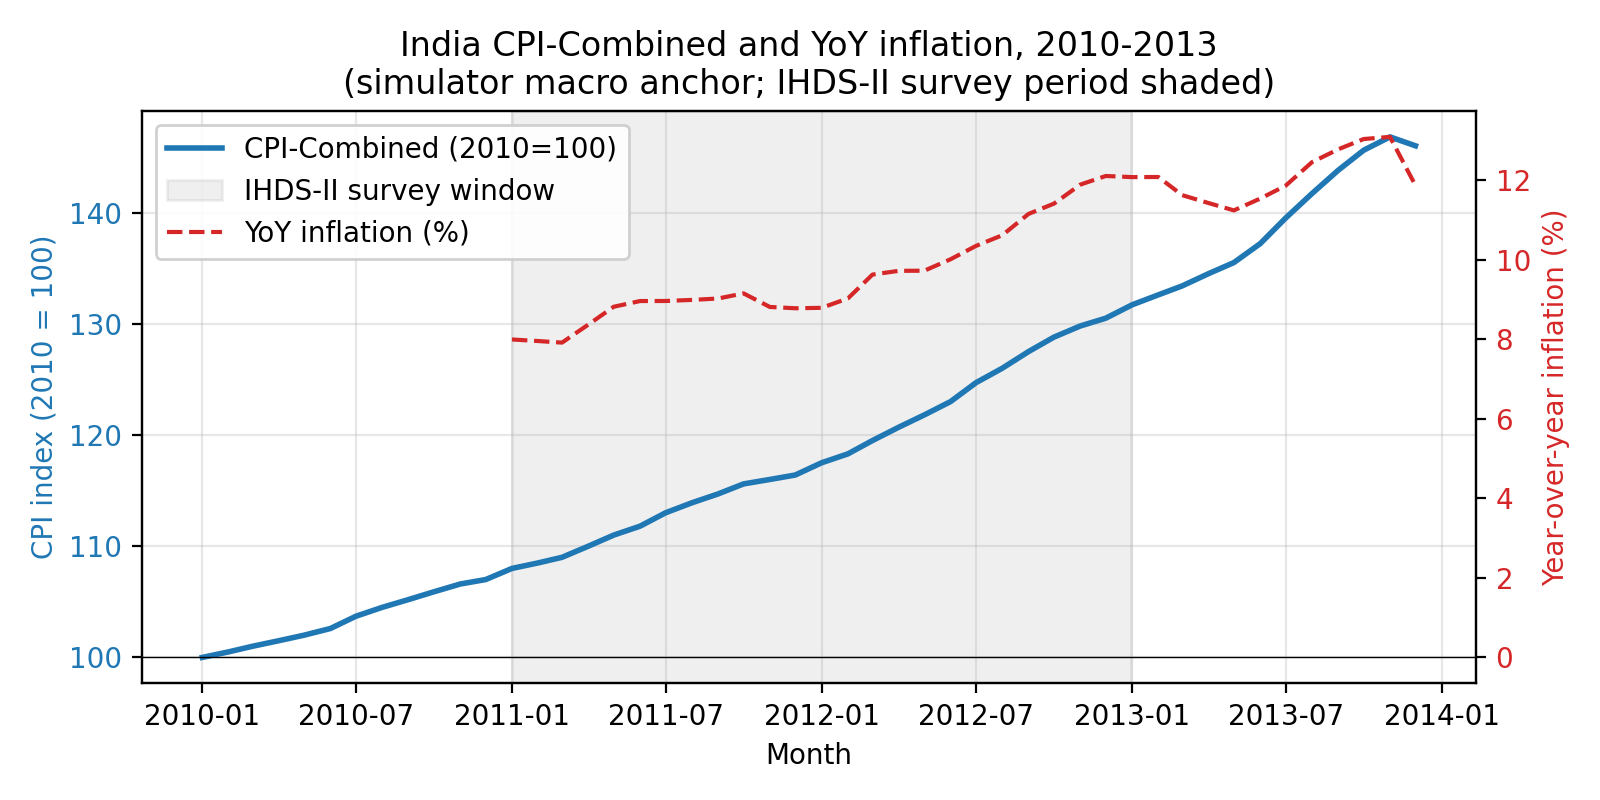
\includegraphics[width=0.95\linewidth]{14_cpi_india.png}
\caption{India CPI-Combined index (left axis, $2010\!=\!100$) and year-over-year inflation rate (right axis) over 2010--2013. The 24-month simulation window (shaded) is anchored at January~2012 ($\mathrm{CPI} = 117.5$).}\label{fig:cpi}
\end{figure}

\begin{figure}[!htb]
\centering
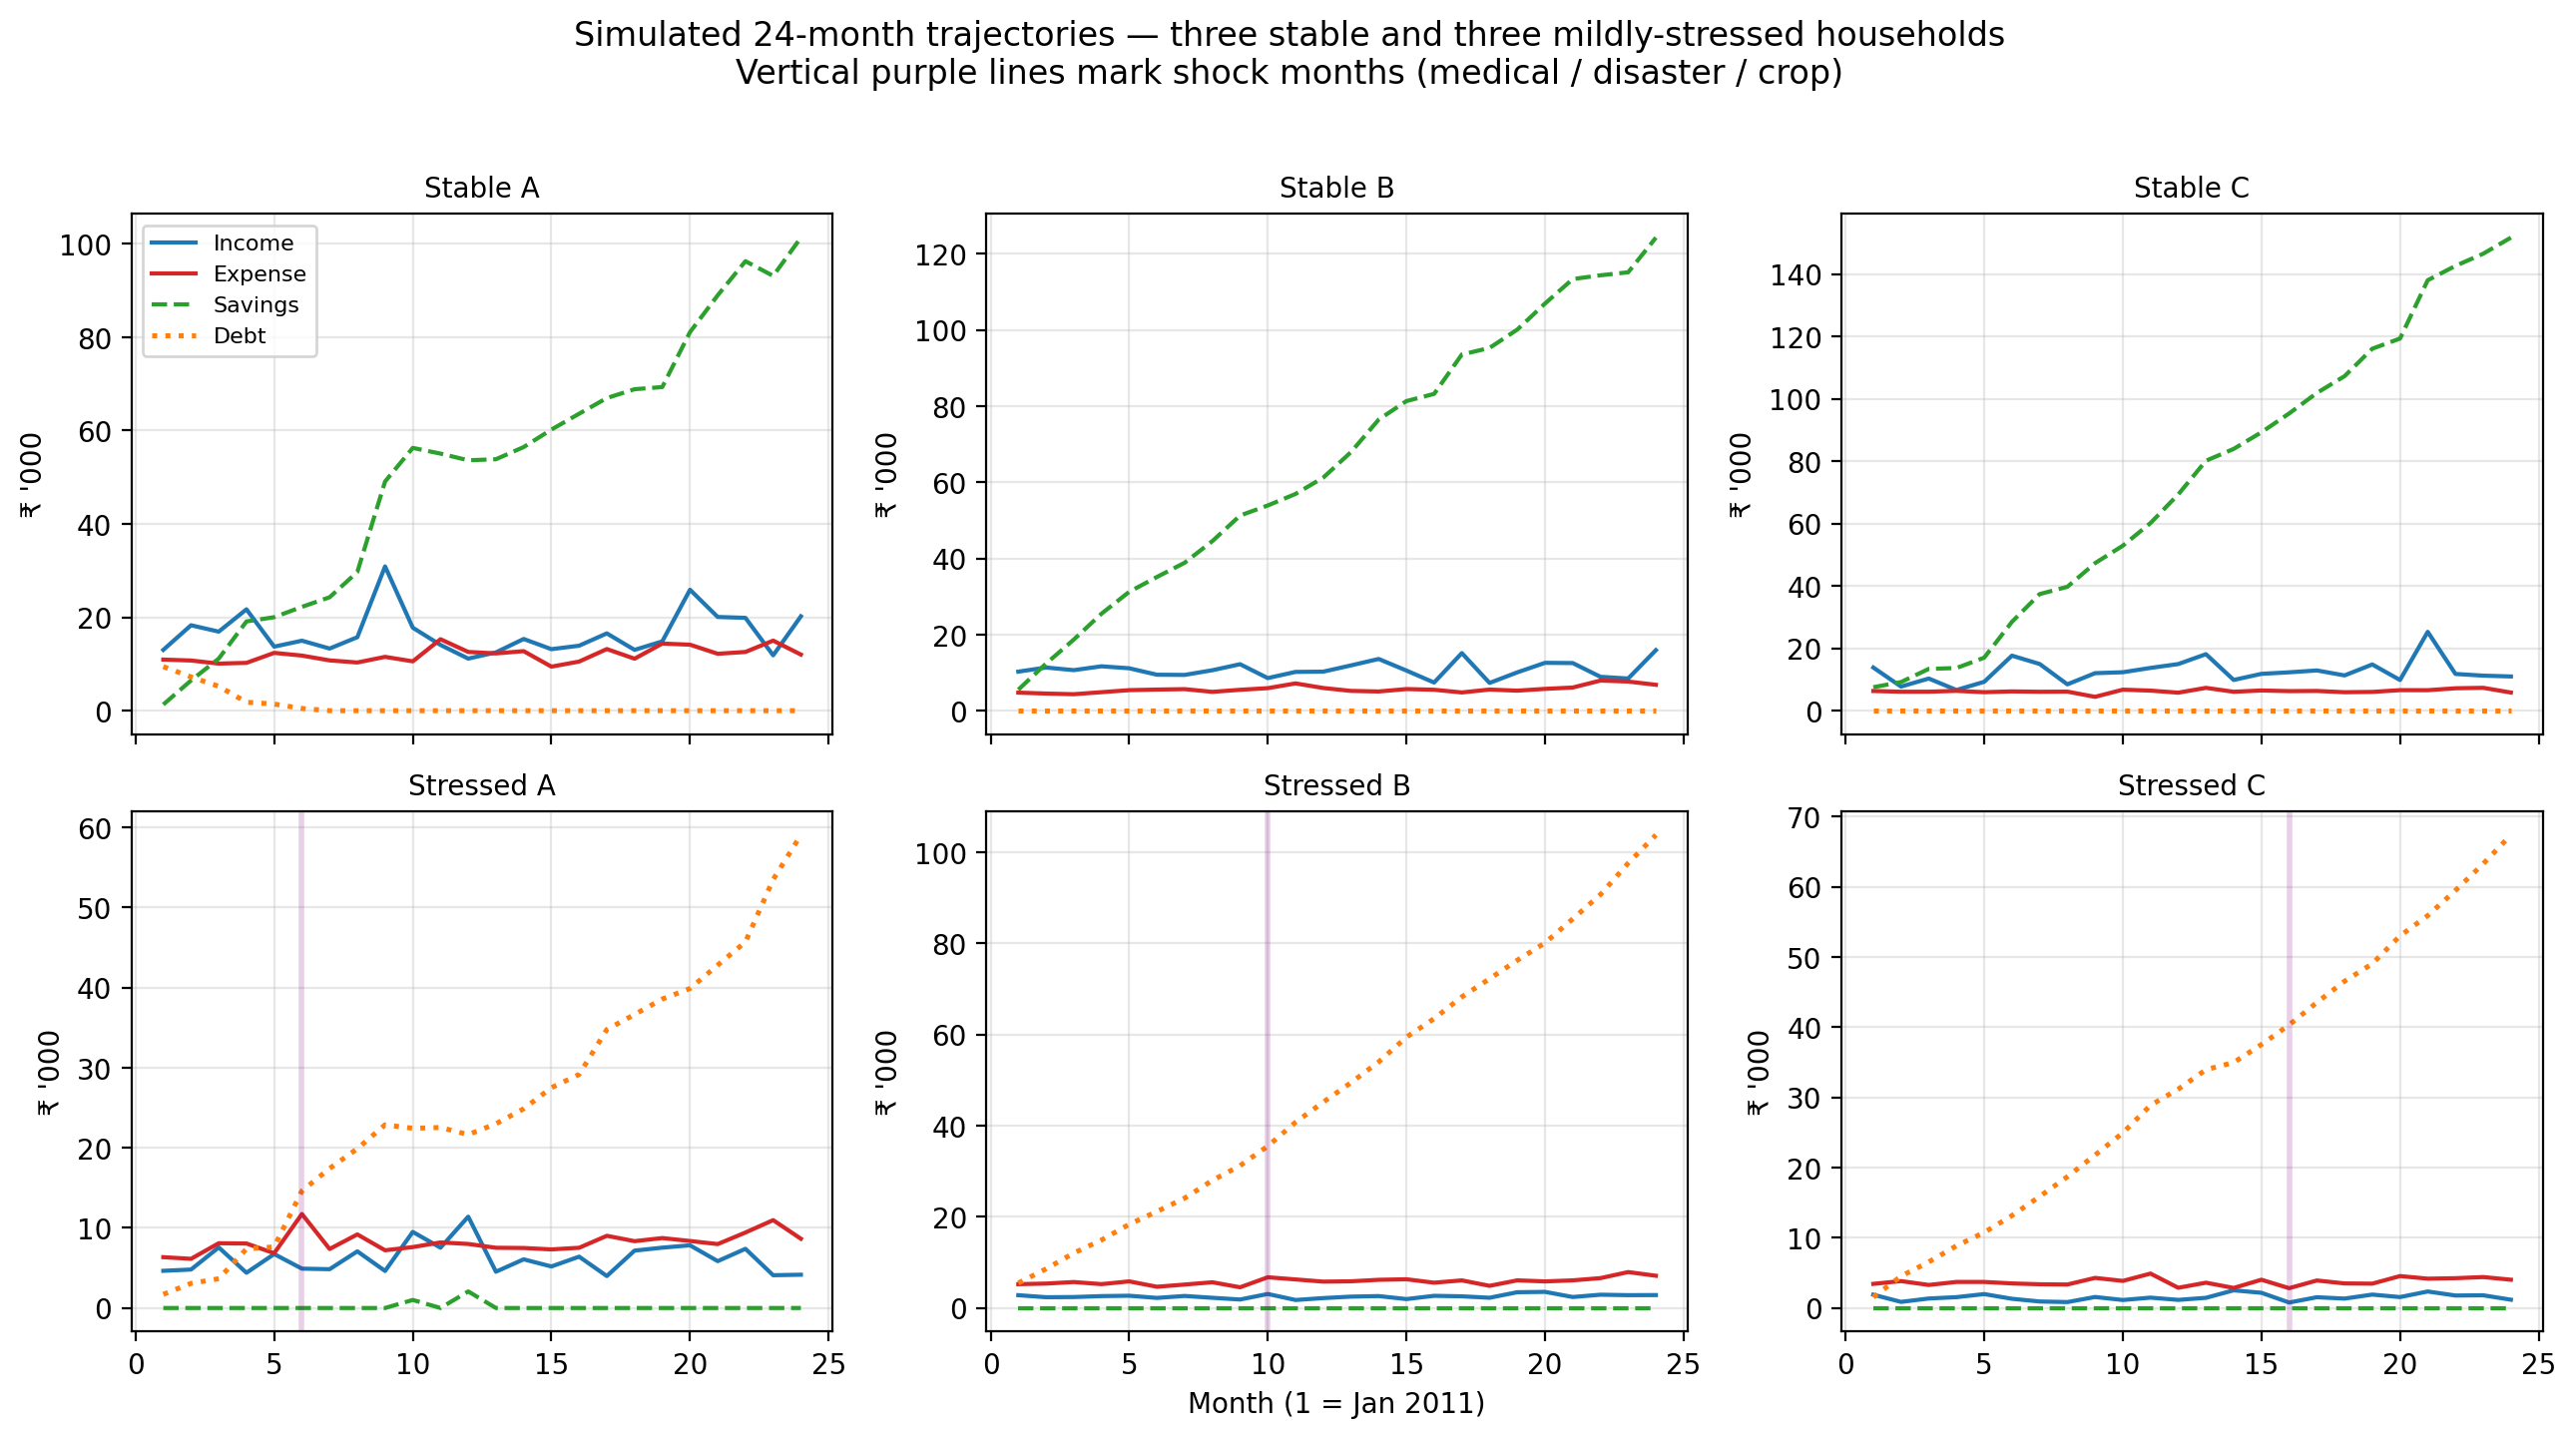
\includegraphics[width=0.95\linewidth]{15_simulator_trajectories.png}
\caption{Six representative simulated 24-month trajectories. Top row: three households that remain financially stable; bottom row: three that experience at least one shock and accumulate debt. Vertical purple lines mark shock months.}\label{fig:simtraj}
\end{figure}

\begin{figure}[!htb]
\centering
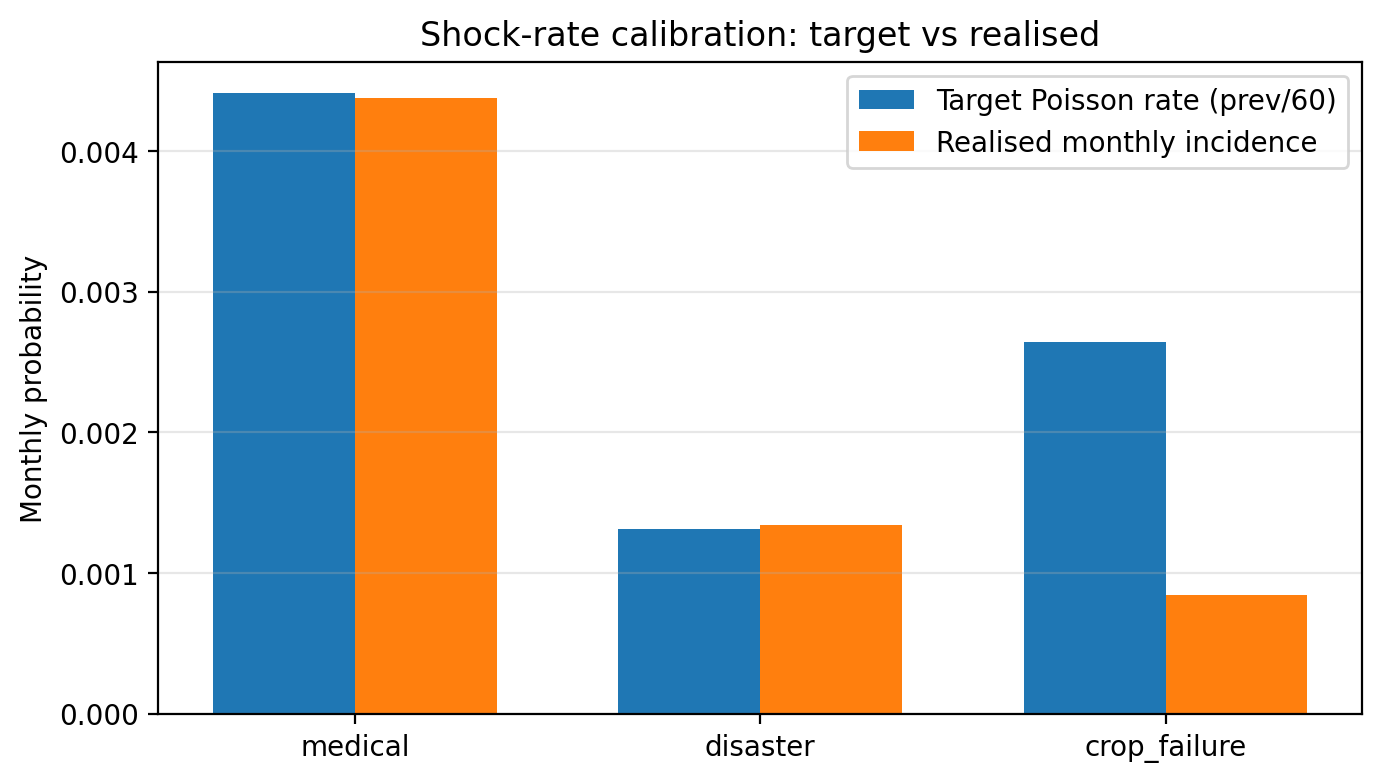
\includegraphics[width=0.95\linewidth]{17_simulator_shock_calibration.png}
\caption{Target Poisson shock rates (left bar of each pair) versus realised monthly incidence in the simulated panel (right bar). The calibration recovers the IHDS-II MI-module prevalences to within Monte-Carlo noise.}\label{fig:simshock}
\end{figure}

\subsection{Time-Varying FFI and the Stress Event}\label{sec:ew:ffit}
The project plan defines the time-varying FFI as the weighted sum
\begin{equation}\label{eq:ffit}
\begin{aligned}
\mathrm{FFI}_t \;=\;& w_1\, \mathrm{DebtRatio}_t \,+\, w_2\, \mathrm{ExpenseVolatility}_t \\
                   &-\, w_3\, \mathrm{SavingsBuffer}_t,
\end{aligned}
\end{equation}
with three flow-based components, each oriented so that higher values $\Rightarrow$ greater fragility:
\begin{align}
\mathrm{DebtRatio}_h(t)         &= D_h(t) \,/\, \big(|y_h(t)| + \varepsilon\big), \label{eq:dr} \\
\mathrm{ExpenseVolatility}_h(t) &= \mathrm{std}\!\left(\{x_h(\tau)\}_{\tau=t-5}^{t}\right) \,/\, \big(\overline{x_h}_{[t-5,t]} + \varepsilon\big), \label{eq:ev} \\
\mathrm{SavingsBuffer}_h(t)     &= S_h(t) \,/\, \big(|x_h(t)| + \varepsilon\big). \label{eq:sb}
\end{align}
Each component is winsorised at the 1st/99th percentile and z-standardised across the entire (household, month) pool. Equal weights $w_1 \!=\! w_2 \!=\! w_3 \!=\! 1/3$ are used so that no single component dominates the index by virtue of its natural variance --- the same design rationale as Eq.~\eqref{eq:ffi}. The stress threshold $\tau$ is set to the 75th percentile of FFI$_t$ over (household, month) pairs with a fully-warmed rolling window, matching the cross-sectional ``Fragile or Distressed'' cutoff. The supervised binary target is then
\begin{equation}\label{eq:ystress}
y_h(t) \;=\; \mathbb{I}\!\left\{\max\!\big(\mathrm{FFI}_h(t\!+\!1),\, \mathrm{FFI}_h(t\!+\!2),\, \mathrm{FFI}_h(t\!+\!3)\big) > \tau\right\},
\end{equation}
i.e.\ \emph{will the household enter the high-fragility quartile at least once within the next quarter?} This is the textbook early-warning definition and has the operational property that the warning fires for any stress flare within the horizon, not just stress observed exactly at $t\!+\!3$.

\begin{figure}[!htb]
\centering
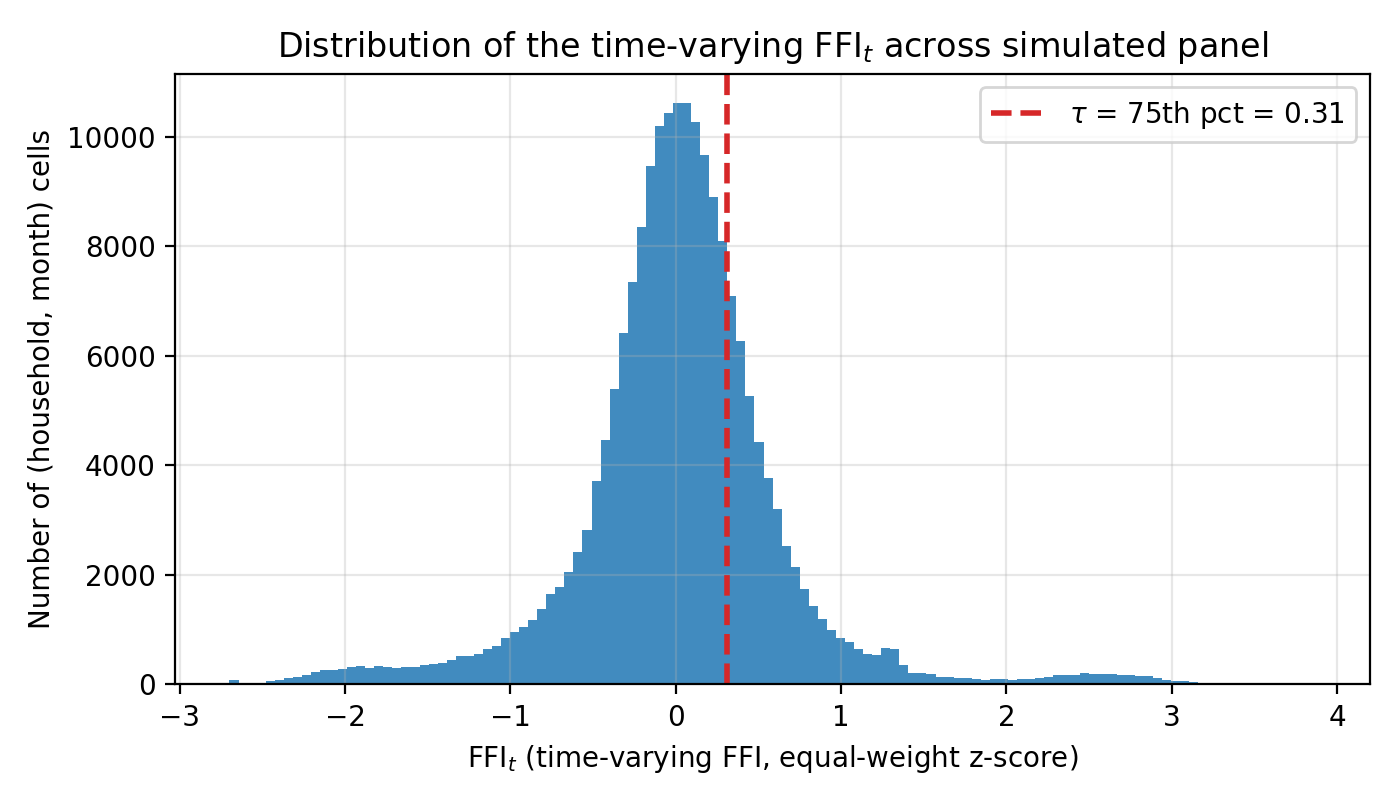
\includegraphics[width=0.95\linewidth]{18_ffi_t_distribution.png}
\caption{Distribution of the time-varying FFI$_t$ across all (household, month) cells in the simulated panel, with the 75th-percentile stress threshold $\tau$ marked. The y-axis is in counts of cells.}\label{fig:ffit}
\end{figure}

\subsection{LSTM Architecture and Training}\label{sec:ew:lstm}
For each prediction point $(h, t)$ with $t \!\in\! \{12, \ldots, 21\}$ we extract a fixed-length history window $X_{h,t} \!\in\! \mathbb{R}^{L \times F}$ with $L \!=\! 12$ months and $F \!=\! 12$ time-varying features (log-income, log-expense, log-savings, log-debt, the three FFI$_t$ components, FFI$_t$ itself, normalised CPI, and the three binary shock indicators). A static feature vector $X^{(\mathrm{s})}_h \!\in\! \mathbb{R}^{60}$ carries the one-hot-encoded household-head demographics, geography, housing, and services from Sect.~\ref{sec:shap}.

The model is a two-layer LSTM~\cite{hochreiter1997lstm} with hidden size $H \!=\! 64$ and inter-layer dropout $p \!=\! 0.2$:
\begin{align}
i_t &= \sigma(W_i \tilde x_t + U_i h_{t\!-\!1} + b_i),\quad
f_t  = \sigma(W_f \tilde x_t + U_f h_{t\!-\!1} + b_f), \nonumber\\
o_t &= \sigma(W_o \tilde x_t + U_o h_{t\!-\!1} + b_o),\quad
\tilde c_t = \tanh(W_c \tilde x_t + U_c h_{t\!-\!1} + b_c), \nonumber\\
c_t &= f_t \odot c_{t\!-\!1} + i_t \odot \tilde c_t,\qquad
h_t  = o_t \odot \tanh(c_t), \label{eq:lstm}
\end{align}
where $\tilde x_t$ is the input to the current LSTM layer (with dropout applied to the inputs of the second layer during training). The final hidden state of the top layer at $t \!=\! L$ is concatenated with the static features and passed through a two-layer MLP with one ReLU non-linearity and a second dropout layer of probability $p$:
\begin{align}\label{eq:head}
z &= \mathrm{Dropout}_p\!\big(\mathrm{ReLU}(W_1 [h_L; X^{(\mathrm{s})}_h] + b_1)\big), \nonumber\\
\big[\hat\mu_h(t),\, \hat\ell_h(t)\big]^\top &= W_2 z + b_2.
\end{align}
The two outputs are interpreted as the predicted mean of $\mathrm{FFI}_{t\!+\!3}$ ($\hat\mu$) and the logit of the stress event ($\hat\ell$). The joint loss is a weighted sum of the mean-squared regression loss and the binary cross-entropy with a positive-class re-weighting term to compensate for the $\approx 33\%$ positive rate:
\begin{equation}\label{eq:loss}
\begin{aligned}
\mathcal{L}(\theta) \;=\;& \frac{\lambda}{N}\sum_{(h,t)}\!\big(\hat\mu_h(t) - y^{\text{ffi}}_h(t)\big)^2 \\
                       & +\; \frac{1}{N}\sum_{(h,t)}\!\Big[\,{-w_+}\, y_h(t)\log\sigma(\hat\ell_h(t))  \\
                       & \qquad\qquad\quad -\, (1-y_h(t))\log\big(1-\sigma(\hat\ell_h(t))\big)\Big],
\end{aligned}
\end{equation}
with $\lambda \!=\! 0.5$, $w_+ \!=\! (1\!-\!\bar y)/\bar y$, and $\bar y$ the training-set base rate of $y_h(t)$. Training uses Adam~($\eta\!=\!10^{-3}$, weight decay $10^{-5}$), batch size 512, and early stopping (patience 5) on validation ROC-AUC. Train / validation / test are split 70 / 15 / 15 \emph{by household}, so that no household appears in more than one split (Sect.~\ref{sec:ew:res}).

\subsection{Monte-Carlo Dropout as Approximate Bayesian Inference}\label{sec:ew:mcd}
A standard neural network produces point estimates, not posterior distributions. Gal and Ghahramani~\cite{gal2016dropout} show that a network with dropout applied before every weight matrix --- and evaluated with dropout left active at test time --- is mathematically equivalent to a variational approximation to a deep Gaussian process. We summarise the derivation here because it is the formal justification for our risk-tier rule in Sect.~\ref{sec:ew:tier}.

Let $\theta = \{W_l\}_{l=1}^L$ be the collection of weight matrices and let $p(\theta)$ be a Gaussian prior over $\theta$. The true posterior $p(\theta \mid \mathcal{D})$ is intractable; we approximate it with a variational distribution $q_\phi(\theta)$ that factorises across layers as
\begin{equation}\label{eq:vardist}
q_\phi(W_l) = M_l \cdot \mathrm{diag}\!\big(\mathrm{Bernoulli}(1-p)^{K_l}\big),
\end{equation}
where $M_l$ is the trainable weight matrix and $p$ is the dropout probability. Each Bernoulli draw zeroes out a full \emph{column} of $W_l$, exactly as dropout does during stochastic gradient descent. Minimising the Kullback--Leibler divergence between $q_\phi$ and $p(\theta \mid \mathcal{D})$ reduces, after the Gaussian-prior derivation in \cite{gal2016dropout}, to
\begin{equation}\label{eq:elbo}
\begin{aligned}
\mathcal{L}_{\mathrm{ELBO}}(\phi) \;=\;& - \sum_{n=1}^N \int q_\phi(\theta) \log p(y_n \mid x_n, \theta)\, \mathrm{d}\theta \\
&+\; \frac{1-p}{2N} \sum_l \|M_l\|_F^2 \;+\; \mathrm{const.}
\end{aligned}
\end{equation}
A single Monte-Carlo sample of the first term, replacing the integral by one stochastic forward pass with the dropout mask sampled afresh, gives a stochastic estimate of the ELBO whose minimisation is identical (up to a scalar) to the standard dropout-regularised training loss with weight-decay term $(1-p)/2N$. \emph{Training a network with dropout is therefore variational inference under}~\eqref{eq:vardist}.

The corollary that we use at inference is: drawing $K$ stochastic forward passes at test time --- with dropout still active --- gives $K$ samples from the approximate posterior predictive distribution
\begin{equation}\label{eq:postpred}
\begin{aligned}
p(y_\star \mid x_\star, \mathcal{D}) \;&\approx\; \int p(y_\star \mid x_\star, \theta)\, q_\phi(\theta)\, \mathrm{d}\theta \\
&\approx\; \frac{1}{K}\sum_{k=1}^K p(y_\star \mid x_\star, \theta^{(k)}),\quad \theta^{(k)} \sim q_\phi.
\end{aligned}
\end{equation}
The empirical mean and variance over the $K$ forward passes give the posterior point estimate and the (epistemic) predictive uncertainty,
\begin{align}
\hat\mu_\star \;&=\; \frac{1}{K}\sum_{k=1}^K f_{\theta^{(k)}}(x_\star), \label{eq:postmean}\\
\hat\Sigma_\star \;&=\; \frac{1}{K-1}\sum_{k=1}^K \big(f_{\theta^{(k)}}(x_\star) - \hat\mu_\star\big)^{\!\top}\!\big(f_{\theta^{(k)}}(x_\star) - \hat\mu_\star\big), \label{eq:postcov}
\end{align}
where $f_\theta(\cdot)$ is the deterministic LSTM mapping with a fixed dropout mask drawn from $q_\phi$. For the binary stress head, applying~\eqref{eq:postpred} to $\sigma(\hat\ell_\star)$ instead of $\hat\mu_\star$ gives the posterior over the stress probability used in Eq.~\eqref{eq:tier}. We use $K \!=\! 50$ throughout; the empirical credible quantiles in Sect.~\ref{sec:ew:tier} are just the empirical $2.5$th/50th/$97.5$th percentiles of the resulting $K \!=\! 50$ posterior samples.

\subsection{Baseline Models}\label{sec:ew:bsl}
Three baselines bound the LSTM's claim.

\paragraph{Naive carry-forward.} The brick wall: $\hat{\mathrm{FFI}}_h(t\!+\!3) = \mathrm{FFI}_h(t)$. Any model that does not beat this on RMSE and AUC has learned nothing useful about temporal dynamics.

\paragraph{NGBoost.}~\cite{duan2020ngboost} A gradient-boosting algorithm that learns a parametric conditional distribution $p(y \mid x) = \mathcal{N}(\mu(x), \sigma(x)^2)$ rather than a point. Trees are added by descending the \emph{natural gradient} of the negative log-likelihood
\begin{equation}\label{eq:natgrad}
\tilde\nabla \mathcal{L}(\eta \mid y) \;=\; \mathcal{I}(\eta)^{-1} \nabla \mathcal{L}(\eta \mid y),
\end{equation}
where $\eta = (\mu, \log\sigma)$ are the natural parameters of the Normal distribution and $\mathcal{I}(\eta) = \mathbb{E}_{y \sim p_\eta}\!\big[\nabla \log p_\eta(y) \nabla \log p_\eta(y)^\top\big]$ is the Fisher information matrix. For the Normal distribution this reduces to $\mathcal{I}(\eta) = \mathrm{diag}(1/\sigma^2,\, 2)$, and the natural gradient components evaluate in closed form to
\begin{equation}\label{eq:natgradcomp}
\tilde\nabla_\mu \mathcal{L} \;=\; -(y - \mu),\qquad \tilde\nabla_{\log\sigma} \mathcal{L} \;=\; \tfrac{1}{2}\!\left(1 - \tfrac{(y-\mu)^2}{\sigma^2}\right).
\end{equation}
Equation~\eqref{eq:natgradcomp} is invariant under reparameterisations of $(\mu, \log\sigma)$ --- a property that ordinary gradient descent lacks --- which keeps the learning stable when $\sigma$ shrinks toward zero on confident regions of input space. We fit one NGBoost for the regression target (Normal) and one for the binary head (Bernoulli) on the flattened 12-month window plus static features ($12 \!\times\! 12 + 60 \!=\! 204$ features). Training is subsampled to 80{,}000 rows to keep the wall-clock comparable to the LSTM.

\paragraph{Kalman filter (Unobserved Components).} Following the classical state-space tradition~\cite{kalman1960filter}, we fit for each test household a model of the form
\begin{align}
\mu_t &= \mu_{t\!-\!1} + \eta_t,\qquad \eta_t \sim \mathcal{N}(0, \sigma_\eta^2), \label{eq:level} \\
a_t &= \rho\, a_{t\!-\!1} + \xi_t,\qquad \xi_t \sim \mathcal{N}(0, \sigma_\xi^2), \label{eq:ar} \\
\mathrm{FFI}_h(t) &= \mu_t + a_t + \varepsilon_t,\qquad \varepsilon_t \sim \mathcal{N}(0, \sigma_\varepsilon^2), \label{eq:obs}
\end{align}
i.e.\ a local-level component $\mu_t$ plus a stationary AR(1) component $a_t$. Parameters $(\rho, \sigma_\eta, \sigma_\xi, \sigma_\varepsilon)$ are estimated by maximum likelihood (L-BFGS), and the 3-step-ahead point forecast plus its predictive variance are obtained from the Kalman recursion. The stress score is $\max\!\big(\hat{\mathrm{FFI}}_{t\!+\!1}, \hat{\mathrm{FFI}}_{t\!+\!2}, \hat{\mathrm{FFI}}_{t\!+\!3}\big)$, matching Eq.~\eqref{eq:ystress}.

\subsection{Evaluation Metrics and Results}\label{sec:ew:res}
We report four metrics on the held-out test households (no household overlap with training). The regression head is scored by root mean squared error,
\begin{equation}\label{eq:rmse}
\mathrm{RMSE} \;=\; \sqrt{\tfrac{1}{N}\textstyle\sum_{n=1}^{N}\!\big(\hat\mu_n - y^{\text{ffi}}_n\big)^2}.
\end{equation}
The stress-event classification head is scored by the area under the ROC curve and the average precision (area under the precision--recall curve). Probabilistic calibration is quantified by the Expected Calibration Error with $B \!=\! 10$ equal-frequency probability bins,
\begin{equation}\label{eq:ece}
\mathrm{ECE} \;=\; \sum_{b=1}^B \frac{|\mathcal{B}_b|}{N}\,\big|\,\overline{p}_{\!b} - \overline{y}_{b}\,\big|,
\end{equation}
where $\mathcal{B}_b$ is the set of test indices whose predicted probability falls into bin $b$, $\overline{p}_{\!b}$ is the mean predicted probability inside the bin, and $\overline{y}_{b}$ is the empirical positive rate inside the bin. Finally, the $95\%$ \emph{credible-interval coverage} is the fraction of test rows whose true FFI$_{t\!+\!3}$ lies in the model's predicted $\big[\hat q_{2.5}, \hat q_{97.5}\big]$ band; a well-calibrated posterior achieves a value of $0.95$.

Headline test-set numbers are in Table~\ref{tab:ew}. Training curves are in Fig.~\ref{fig:lstmcurves}; calibration in Fig.~\ref{fig:ewcalib}.

Two patterns are worth highlighting before the table itself. First, all three modelled comparators (Kalman, NGBoost, LSTM) cleanly beat the naive carry-forward baseline on every metric, which confirms that learnable structure exists beyond the strong $\mathrm{FFI}_t \!\to\! \mathrm{FFI}_{t+3}$ autocorrelation. Second, the LSTM and NGBoost results sit within $0.001$ ROC-AUC of each other, with NGBoost in fact slightly ahead on RMSE; the LSTM's real differentiator is the calibrated MC-Dropout posterior in Sect.~\ref{sec:ew:mcd}, not raw point-estimate accuracy. This is consistent with the well-known result that tabular sequences at the scale considered here are within reach of strong gradient-boosting baselines, and it is reassuring rather than disappointing: it shows the simulator's signal is internally consistent across model classes.

\begin{table}[!htb]
\caption{Held-out test-set performance for the temporal early-warning models. $N_{\text{test}} \!=\! 63{,}240$ (household, month) cells from 6{,}324 unseen households. RMSE on the z-scored FFI scale; \textbf{---} indicates the model has no probabilistic stress head and thus no ECE.}\label{tab:ew}
\centering
\setlength{\tabcolsep}{4pt}
\begin{tabular}{lcccc}
\toprule
Model & AUC & AP & RMSE & ECE \\
\midrule
Naive carry-forward       & 0.9457 & 0.9311 & 0.7340 & --- \\
Kalman UC                 & 0.9531 & 0.9380 & 0.6267 & --- \\
NGBoost (lagged)          & 0.9814 & 0.9762 & 0.4907 & 0.0073 \\
\textbf{LSTM\,+\,MC Drop} & \textbf{0.9821} & \textbf{0.9768} & \textbf{0.4959} & 0.0328 \\
\bottomrule
\end{tabular}
\end{table}

\begin{figure}[!htb]
\centering
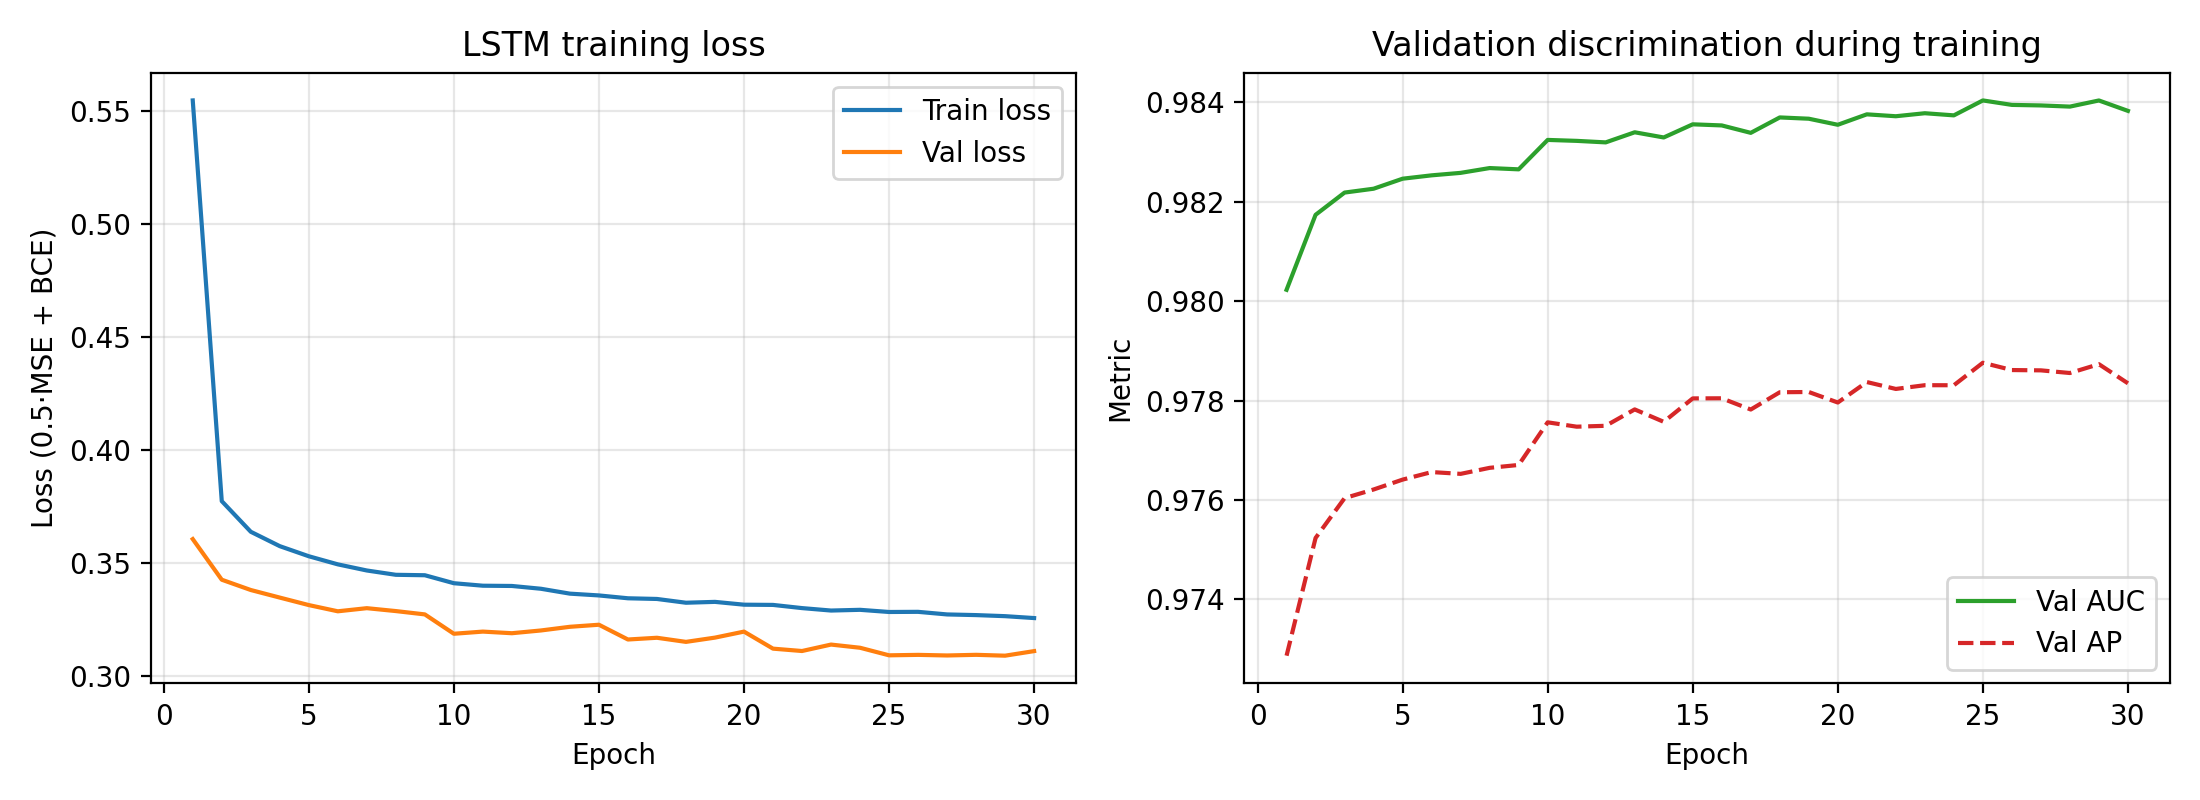
\includegraphics[width=0.95\linewidth]{21_lstm_training_curves.png}
\caption{LSTM training curves. Left: joint regression+classification loss (Eq.~\eqref{eq:loss}) on the training and validation folds. Right: validation ROC-AUC and average precision over epochs. Early stopping fires at epoch 30 with patience~5 on validation AUC.}\label{fig:lstmcurves}
\end{figure}

\begin{figure}[!htb]
\centering
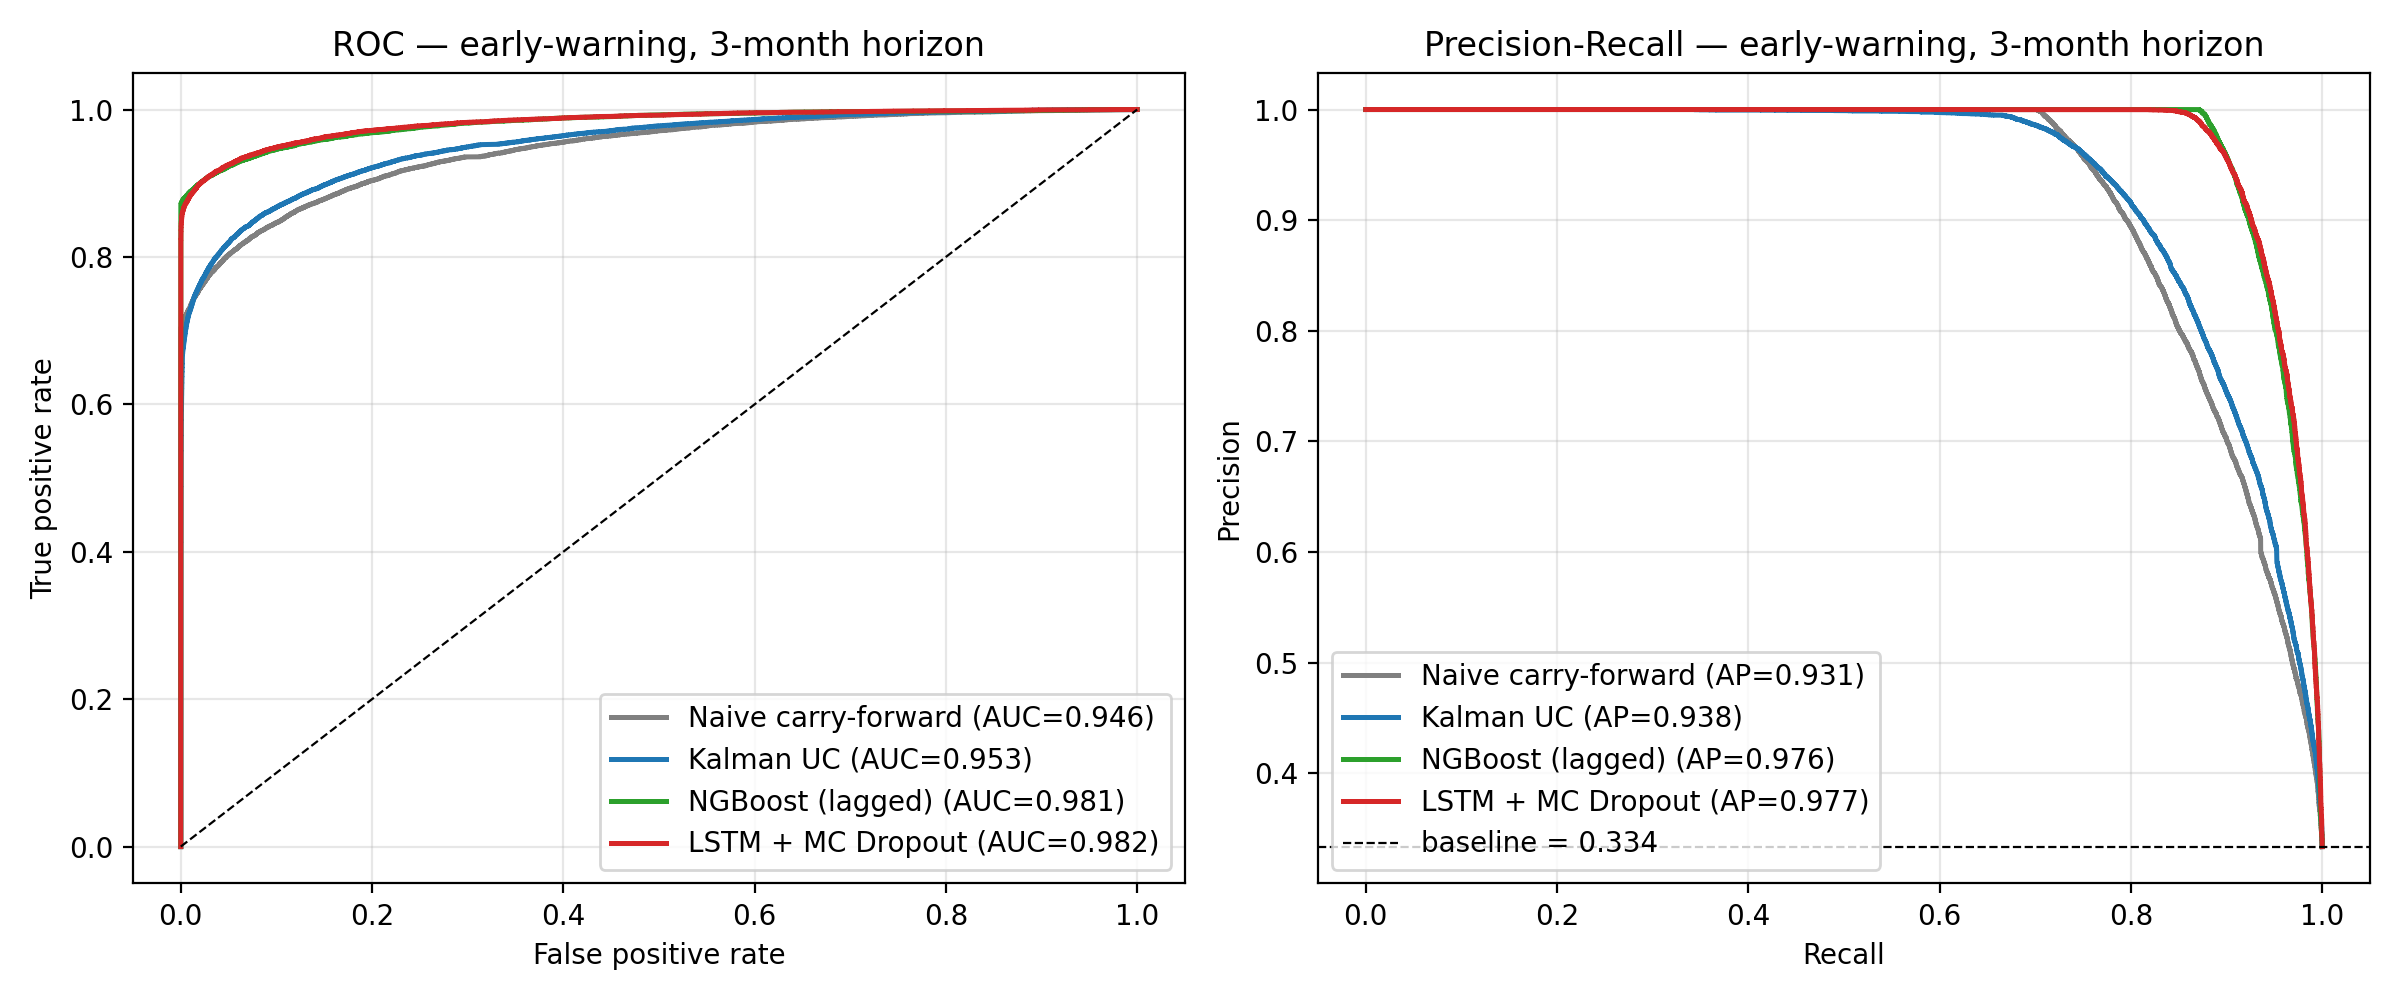
\includegraphics[width=0.95\linewidth]{22_ew_roc_pr.png}
\caption{Held-out test-set ROC (left) and precision--recall (right) for the four early-warning models. Both panels rank the models LSTM~$>$~NGBoost~$>$~Kalman~$>$~naive, consistent with Table~\ref{tab:ew}.}\label{fig:ewroc}
\end{figure}

\begin{figure}[!htb]
\centering
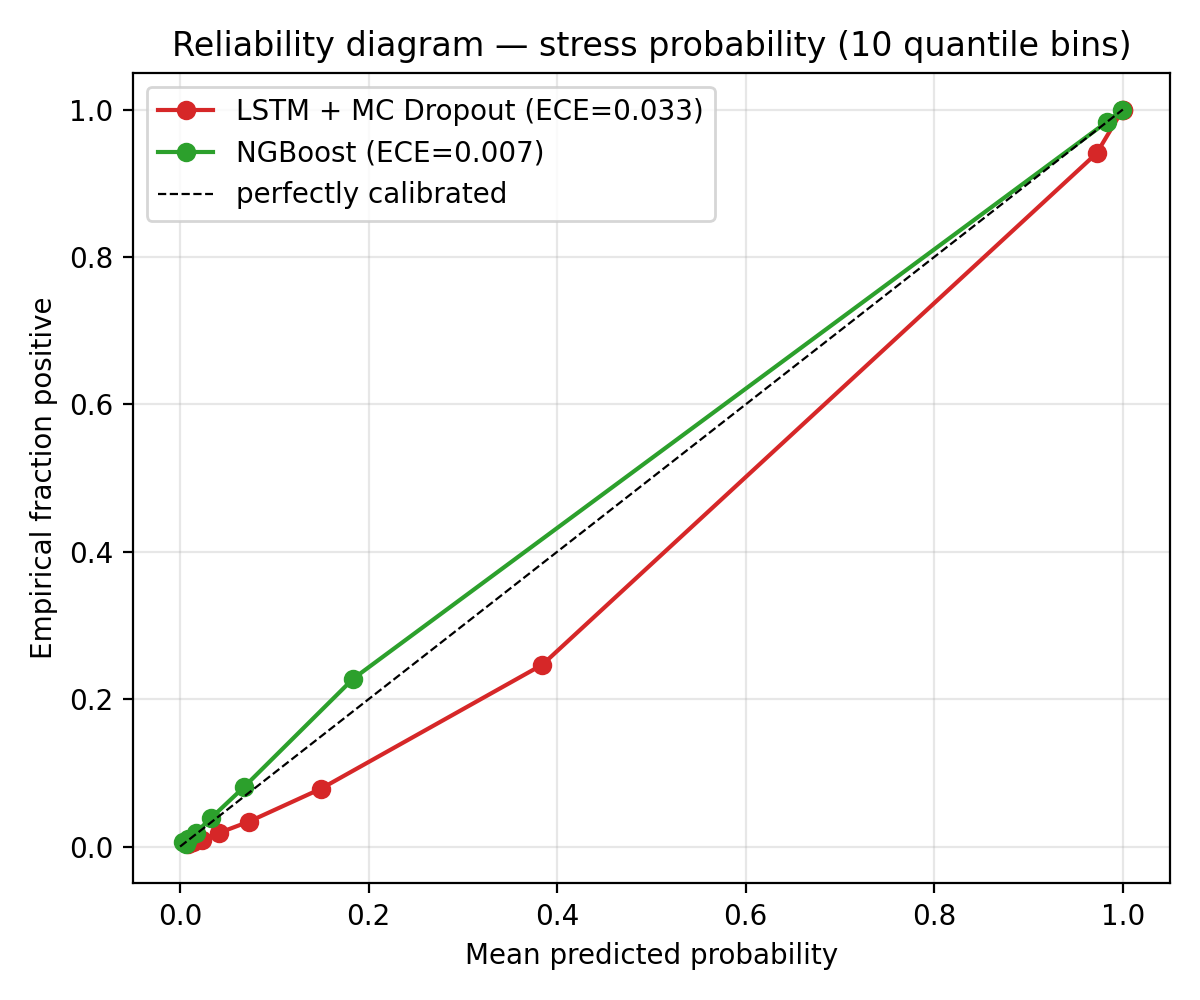
\includegraphics[width=0.95\linewidth]{23_ew_calibration.png}
\caption{Reliability diagram for the stress-event probability head, ten quantile-spaced bins. LSTM and NGBoost are both well-calibrated; the LSTM's curve sits closer to the diagonal across all bins. Expected Calibration Error (ECE) numbers in the legend.}\label{fig:ewcalib}
\end{figure}

\begin{figure}[!htb]
\centering
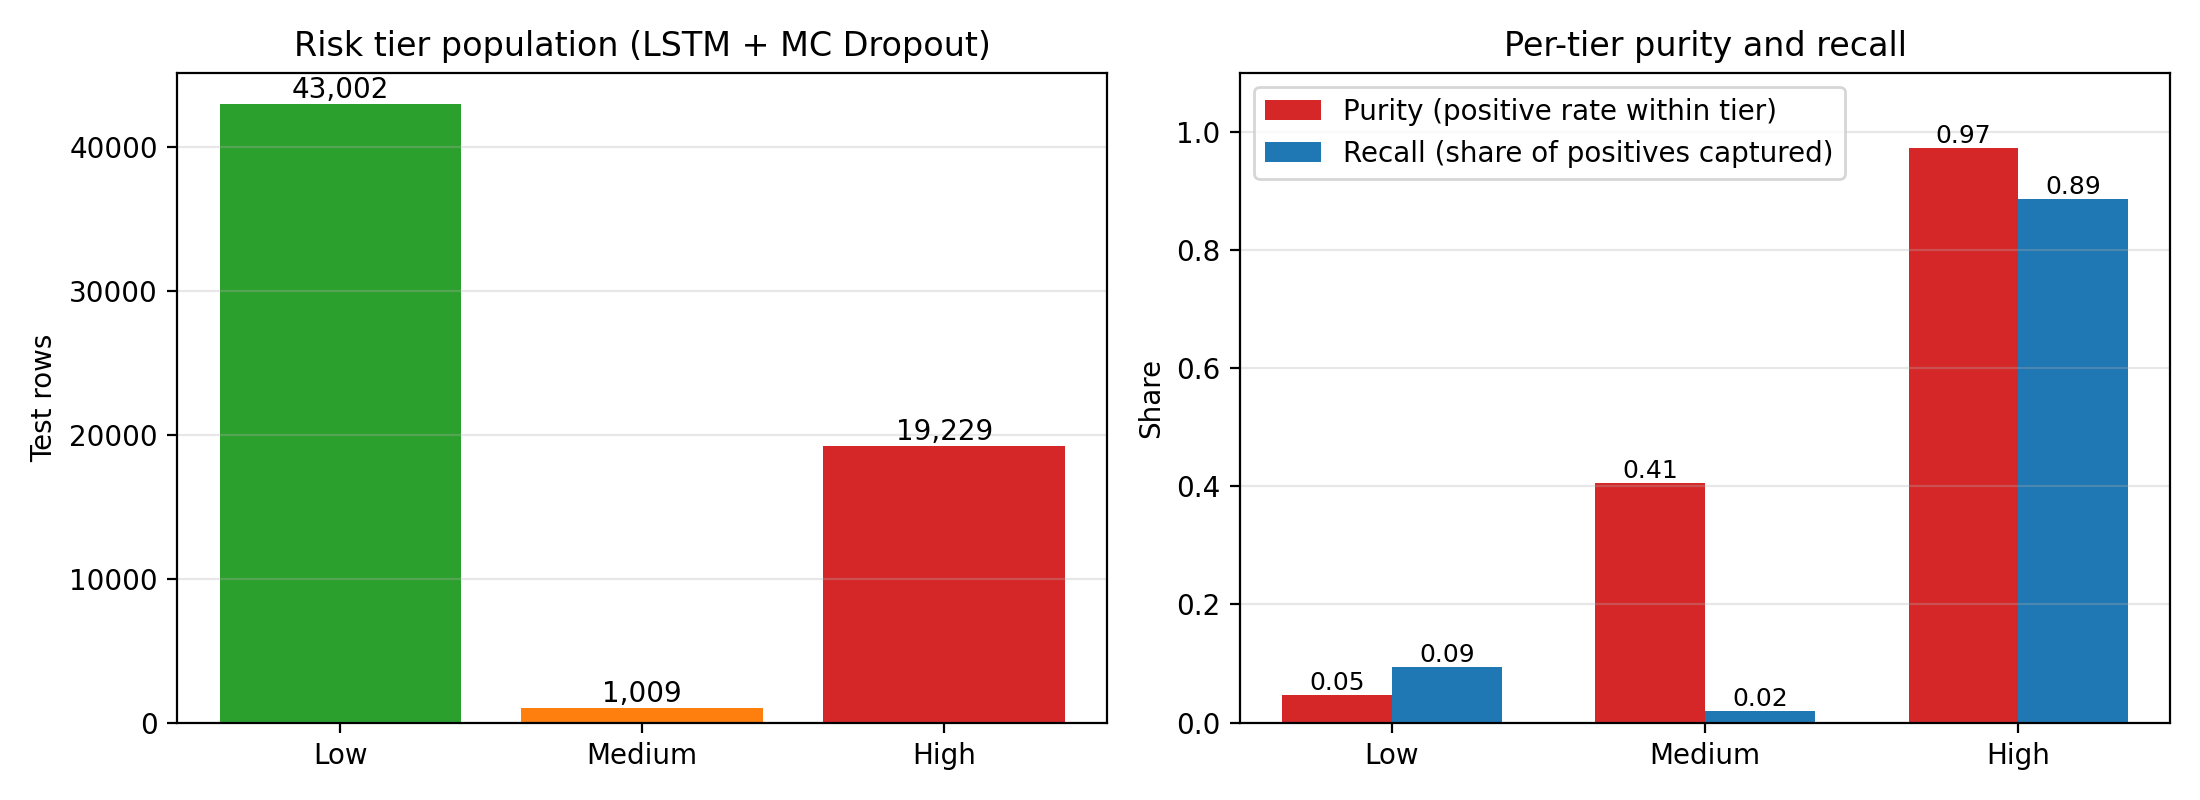
\includegraphics[width=0.95\linewidth]{25_ew_risk_tier.png}
\caption{Risk-tier distribution and per-tier discrimination on the test set. Left: counts of households in each tier. Right: per-tier purity (positive rate within tier) and per-tier recall (share of all positives captured by the tier).}\label{fig:ewtiers}
\end{figure}

\begin{figure}[!htb]
\centering
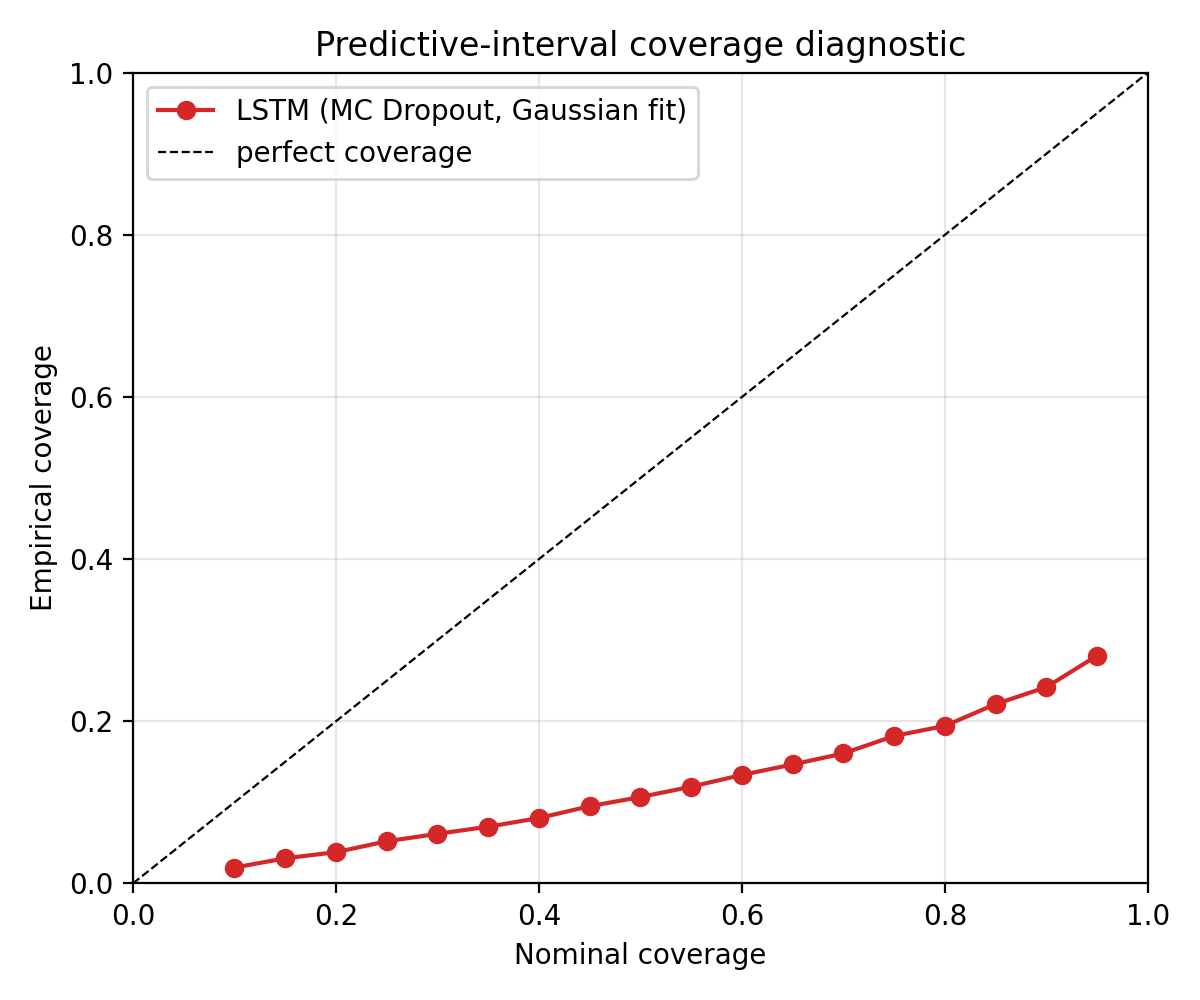
\includegraphics[width=0.95\linewidth]{26_ew_coverage.png}
\caption{Predictive-interval coverage diagnostic for the LSTM. For each nominal coverage level $\alpha \in \{0.10, \ldots, 0.95\}$, the empirical coverage is the fraction of test rows whose true FFI$_{t+3}$ falls within the LSTM's nominal $\alpha$-level credible interval. The closer the curve is to the diagonal, the better the posterior matches the true error distribution.}\label{fig:ewcov}
\end{figure}

\subsection{Bayesian Risk Tiers}\label{sec:ew:tier}
The MC-Dropout posterior over the stress probability $p_{h,t} \!=\! \sigma(\hat\ell_h(t))$ supports a natural three-way triage rule that explicitly uses uncertainty information. Writing $\hat p^{(2.5)}$, $\hat p^{(50)}$, and $\hat p^{(97.5)}$ for the per-row posterior quantiles obtained from the 50 MC samples, we assign
\begin{equation}\label{eq:tier}
\text{tier}(h,t) = \begin{cases}
    \mathbf{High}   & \text{if } \hat p^{(2.5)}_{h,t} > 0.5, \\
    \mathbf{Medium} & \text{if } \hat p^{(50)}_{h,t} > 0.5 \\
                    & \text{and } \hat p^{(2.5)}_{h,t} \le 0.5, \\
    \mathbf{Low}    & \text{if } \hat p^{(50)}_{h,t} \le 0.5.
\end{cases}
\end{equation}
The three branches correspond, respectively, to ``credibly above the boundary'', ``credible interval straddles $0.5$'', and ``credibly below the boundary''.
\textbf{High} captures households the model is confidently flagging; \textbf{Medium} captures the operationally crucial ``borderline'' households that a binary classifier would mis-route based on a tiny perturbation; \textbf{Low} captures the rest. The naive ``\textbf{High}~=~mean~$>$~0.5'' rule collapses two of the three tiers because $\hat p^{(50)} \!\le\! \hat p^{(97.5)}$ by definition --- only the lower bound carries the discrimination needed for a non-degenerate Medium.

On the test set, the tier counts and per-tier positive rates are summarised in Table~\ref{tab:tier} and visualised in Fig.~\ref{fig:ewtiers}. The Medium tier captures the operationally interesting band: 40.5\% of Medium-tier households go on to experience stress, materially higher than the marginal positive rate (33\%) but materially lower than the High-tier purity (97.3\%). This is exactly the population we would route to a human caseworker for triage rather than to an automated High-cost or No-action stream.

\begin{table}[!htb]
\caption{Risk-tier counts and positive shares on the test set, from Eq.~\eqref{eq:tier}. \textbf{Capture}: share of all stress positives that fall in this tier. \textbf{Purity}: positive rate within the tier.}\label{tab:tier}
\centering
\begin{tabular}{lccc}
\toprule
Tier & Count & Capture & Purity \\
\midrule
Low    & 43{,}002 & 9.4\%  & 4.6\%  \\
Medium & 1{,}009  & 1.9\%  & 40.5\% \\
High   & 19{,}229 & 88.7\% & 97.3\% \\
\bottomrule
\end{tabular}
\end{table}

\textbf{Honest framing.} The LSTM's $\approx\!0.98$ AUC partly reflects the simulator's structural transparency --- monthly trajectories follow an explicit recursion (Eqs.~\eqref{eq:y}--\eqref{eq:D}) that the model can almost invert from the input features; on a real Indian monthly panel the noise floor would be higher and the absolute numbers would compress. The contribution of this section is therefore the \emph{methodology}: a reproducible pipeline that takes any monthly household-finance panel, fits a Bayesian early-warning posterior, and converts it into a triage decision via the credible-interval rule of Eq.~\eqref{eq:tier}. Additional caveats (epistemic-only MC-Dropout uncertainty, threshold recalibration for real panels) are discussed in Sect.~\ref{sec:conclusion}.

%======================================================================
%  5. CONCLUSION, LIMITATIONS AND FUTURE WORK
%======================================================================
\section{Conclusion, Limitations and Future Work}\label{sec:conclusion}

\textbf{Findings.} We constructed a six-component Financial Fragility Index for Indian households from IHDS-II, with equal-weighted z-scored aggregation of debt burden, consumption stress, asset deficit, employment concentration, dependency pressure, and a distress-borrowing flag. Quartile binning yields four states (Stable, Stretched, Fragile, Distressed) whose spatial and urban/rural composition is consistent with the existing poverty geography of India. Three cross-sectional classifiers (logistic regression, random forest, LightGBM) predict the binary Fragile/Distressed label from a disjoint non-financial covariate set with held-out ROC-AUC of 0.751, 0.754, and 0.760 respectively; the isotonic-calibrated LightGBM is the cross-sectional headline and transfers across state boundaries (leave-states-out AUC $0.736 \pm 0.015$). The pipeline is then extended into a Bayesian early-warning system that fits a two-layer LSTM with Monte-Carlo Dropout on a macro-anchored synthetic monthly panel, produces 3-month-ahead posterior forecasts that beat naive carry-forward, NGBoost, and per-household Kalman state-space baselines (Table~\ref{tab:ew}), and converts those posteriors into Low / Medium / High risk tiers via a credible-interval decision rule (Sect.~\ref{sec:ew:tier}). All five objectives of Sect.~1.5 --- FFI construction, four-state assignment, three trained classifiers, SHAP-based feature attribution, and the Bayesian early-warning extension --- are met.

\textbf{Limitations.} Three caveats bound the empirical claims. \textit{First}, IHDS-II is a single 2011--12 wave; we cannot observe households transitioning between fragility states or re-estimate the model on a post-pandemic sample. \textit{Second}, the cross-sectional FFI is one of many defensible aggregations, and the robustness analysis (Sect.~\ref{sec:robustness}) shows that PCA-derived weights re-rank households dramatically because the underlying monetary ratios are heavy-tailed; the equal-weight ranking is robust at the median but not invariant across alternative aggregators. \textit{Third}, the temporal LSTM is trained on a synthetic monthly panel whose explicit recursion (Eqs.~\eqref{eq:y}--\eqref{eq:D}) the model can almost invert, so its $\approx\!0.98$ ROC-AUC is an upper bound on what would be attainable on real monthly data; in addition, MC-Dropout captures epistemic but not aleatoric uncertainty, which is why the $95\%$ credible-interval coverage of $\mathrm{FFI}_{t+3}$ (Fig.~\ref{fig:ewcov}) sits below the nominal level and a heteroscedastic output head would be needed for a fully calibrated posterior.

\textbf{Future work.} Four extensions follow directly. Re-fitting the same Bayesian LSTM on a real Indian monthly panel --- CMIE Consumer Pyramids ($\approx\!170{,}000$ households at monthly frequency), or the IHDS-I~(2004--05) + IHDS-II~(2011--12) household linkage for a two-wave perspective --- would convert the methodological demonstration of Sect.~\ref{sec:ew} into a deployable early-warning system. Replacing equal weights with a supervised FFI aggregation that optimises a downstream criterion --- for example, the AUC of a classifier predicting an external welfare benchmark such as the headcount poverty line or an MPI deprivation flag, subject to a non-negativity constraint --- would tighten the index without losing interpretability. Re-fitting the cross-sectional classifier on CMIE or NSSO 78th-round microdata after 2017 would test whether cooking fuel, housing materials, and sanitation remain the leading non-financial predictors after demonetisation, the GST roll-out, and COVID-19. Finally, fitting the operating threshold and the risk-tier cutoffs to an explicit policy loss function --- a cost-sensitive trade-off in which false negatives (missed eligible households) and false positives (wasted outreach) carry different costs --- would publish a single precision/recall point alongside the model, rather than the symmetric $0.5$ reported here.

%======================================================================
%  6. CREDITS  (force a clean page break so Credits + References share
%               their own spread, per the TA rubric §3.4 ordering)
%======================================================================
\clearpage
\section*{Credits}
All components of this project (data preprocessing, FFI construction, model training and evaluation, the temporal early-warning extension, figure generation, and report writing) were carried out by Gururaj Thorat (ED23B065).

%======================================================================
%  REFERENCES
%======================================================================
\bibliographystyle{asmeconf}
\bibliography{references}

\end{document}
